% This is our submission, modified from:
% the file JFP2egui.lhs
% release v1.02, 27th September 2001
%   (based on JFPguide.lhs v1.11 for LaLhs 2.09)
% Copyright (C) 2001 Cambridge University Press

\NeedsTeXFormat{LaTeX2e}

\documentclass{jfp1}

%% ODER: format ==         = "\mathrel{==}"
%% ODER: format /=         = "\neq "
%
%
\makeatletter
\@ifundefined{lhs2tex.lhs2tex.sty.read}%
  {\@namedef{lhs2tex.lhs2tex.sty.read}{}%
   \newcommand\SkipToFmtEnd{}%
   \newcommand\EndFmtInput{}%
   \long\def\SkipToFmtEnd#1\EndFmtInput{}%
  }\SkipToFmtEnd

\newcommand\ReadOnlyOnce[1]{\@ifundefined{#1}{\@namedef{#1}{}}\SkipToFmtEnd}
\usepackage{amstext}
\usepackage{amssymb}
\usepackage{stmaryrd}
\DeclareFontFamily{OT1}{cmtex}{}
\DeclareFontShape{OT1}{cmtex}{m}{n}
  {<5><6><7><8>cmtex8
   <9>cmtex9
   <10><10.95><12><14.4><17.28><20.74><24.88>cmtex10}{}
\DeclareFontShape{OT1}{cmtex}{m}{it}
  {<-> ssub * cmtt/m/it}{}
\newcommand{\texfamily}{\fontfamily{cmtex}\selectfont}
\DeclareFontShape{OT1}{cmtt}{bx}{n}
  {<5><6><7><8>cmtt8
   <9>cmbtt9
   <10><10.95><12><14.4><17.28><20.74><24.88>cmbtt10}{}
\DeclareFontShape{OT1}{cmtex}{bx}{n}
  {<-> ssub * cmtt/bx/n}{}
\newcommand{\tex}[1]{\text{\texfamily#1}}	% NEU

\newcommand{\Sp}{\hskip.33334em\relax}


\newcommand{\Conid}[1]{\mathit{#1}}
\newcommand{\Varid}[1]{\mathit{#1}}
\newcommand{\anonymous}{\kern0.06em \vbox{\hrule\@width.5em}}
\newcommand{\plus}{\mathbin{+\!\!\!+}}
\newcommand{\bind}{\mathbin{>\!\!\!>\mkern-6.7mu=}}
\newcommand{\rbind}{\mathbin{=\mkern-6.7mu<\!\!\!<}}% suggested by Neil Mitchell
\newcommand{\sequ}{\mathbin{>\!\!\!>}}
\renewcommand{\leq}{\leqslant}
\renewcommand{\geq}{\geqslant}
\usepackage{polytable}

%mathindent has to be defined
\@ifundefined{mathindent}%
  {\newdimen\mathindent\mathindent\leftmargini}%
  {}%

\def\resethooks{%
  \global\let\SaveRestoreHook\empty
  \global\let\ColumnHook\empty}
\newcommand*{\savecolumns}[1][default]%
  {\g@addto@macro\SaveRestoreHook{\savecolumns[#1]}}
\newcommand*{\restorecolumns}[1][default]%
  {\g@addto@macro\SaveRestoreHook{\restorecolumns[#1]}}
\newcommand*{\aligncolumn}[2]%
  {\g@addto@macro\ColumnHook{\column{#1}{#2}}}

\resethooks

\newcommand{\onelinecommentchars}{\quad-{}- }
\newcommand{\commentbeginchars}{\enskip\{-}
\newcommand{\commentendchars}{-\}\enskip}

\newcommand{\visiblecomments}{%
  \let\onelinecomment=\onelinecommentchars
  \let\commentbegin=\commentbeginchars
  \let\commentend=\commentendchars}

\newcommand{\invisiblecomments}{%
  \let\onelinecomment=\empty
  \let\commentbegin=\empty
  \let\commentend=\empty}

\visiblecomments

\newlength{\blanklineskip}
\setlength{\blanklineskip}{0.66084ex}

\newcommand{\hsindent}[1]{\quad}% default is fixed indentation
\let\hspre\empty
\let\hspost\empty
\newcommand{\NB}{\textbf{NB}}
\newcommand{\Todo}[1]{$\langle$\textbf{To do:}~#1$\rangle$}

\EndFmtInput
\makeatother
%
%
%
%
%
%
% This package provides two environments suitable to take the place
% of hscode, called "plainhscode" and "arrayhscode". 
%
% The plain environment surrounds each code block by vertical space,
% and it uses \abovedisplayskip and \belowdisplayskip to get spacing
% similar to formulas. Note that if these dimensions are changed,
% the spacing around displayed math formulas changes as well.
% All code is indented using \leftskip.
%
% Changed 19.08.2004 to reflect changes in colorcode. Should work with
% CodeGroup.sty.
%
\ReadOnlyOnce{polycode.fmt}%
\makeatletter

\newcommand{\hsnewpar}[1]%
  {{\parskip=0pt\parindent=0pt\par\vskip #1\noindent}}

% can be used, for instance, to redefine the code size, by setting the
% command to \small or something alike
\newcommand{\hscodestyle}{}

% The command \sethscode can be used to switch the code formatting
% behaviour by mapping the hscode environment in the subst directive
% to a new LaTeX environment.

\newcommand{\sethscode}[1]%
  {\expandafter\let\expandafter\hscode\csname #1\endcsname
   \expandafter\let\expandafter\endhscode\csname end#1\endcsname}

% "compatibility" mode restores the non-polycode.fmt layout.

\newenvironment{compathscode}%
  {\par\noindent
   \advance\leftskip\mathindent
   \hscodestyle
   \let\\=\@normalcr
   \let\hspre\(\let\hspost\)%
   \pboxed}%
  {\endpboxed\)%
   \par\noindent
   \ignorespacesafterend}

\newcommand{\compaths}{\sethscode{compathscode}}

% "plain" mode is the proposed default.
% It should now work with \centering.
% This required some changes. The old version
% is still available for reference as oldplainhscode.

\newenvironment{plainhscode}%
  {\hsnewpar\abovedisplayskip
   \advance\leftskip\mathindent
   \hscodestyle
   \let\hspre\(\let\hspost\)%
   \pboxed}%
  {\endpboxed%
   \hsnewpar\belowdisplayskip
   \ignorespacesafterend}

\newenvironment{oldplainhscode}%
  {\hsnewpar\abovedisplayskip
   \advance\leftskip\mathindent
   \hscodestyle
   \let\\=\@normalcr
   \(\pboxed}%
  {\endpboxed\)%
   \hsnewpar\belowdisplayskip
   \ignorespacesafterend}

% Here, we make plainhscode the default environment.

\newcommand{\plainhs}{\sethscode{plainhscode}}
\newcommand{\oldplainhs}{\sethscode{oldplainhscode}}
\plainhs

% The arrayhscode is like plain, but makes use of polytable's
% parray environment which disallows page breaks in code blocks.

\newenvironment{arrayhscode}%
  {\hsnewpar\abovedisplayskip
   \advance\leftskip\mathindent
   \hscodestyle
   \let\\=\@normalcr
   \(\parray}%
  {\endparray\)%
   \hsnewpar\belowdisplayskip
   \ignorespacesafterend}

\newcommand{\arrayhs}{\sethscode{arrayhscode}}

% The mathhscode environment also makes use of polytable's parray 
% environment. It is supposed to be used only inside math mode 
% (I used it to typeset the type rules in my thesis).

\newenvironment{mathhscode}%
  {\parray}{\endparray}

\newcommand{\mathhs}{\sethscode{mathhscode}}

% texths is similar to mathhs, but works in text mode.

\newenvironment{texthscode}%
  {\(\parray}{\endparray\)}

\newcommand{\texths}{\sethscode{texthscode}}

% The framed environment places code in a framed box.

\def\codeframewidth{\arrayrulewidth}
\RequirePackage{calc}

\newenvironment{framedhscode}%
  {\parskip=\abovedisplayskip\par\noindent
   \hscodestyle
   \arrayrulewidth=\codeframewidth
   \tabular{@{}|p{\linewidth-2\arraycolsep-2\arrayrulewidth-2pt}|@{}}%
   \hline\framedhslinecorrect\\{-1.5ex}%
   \let\endoflinesave=\\
   \let\\=\@normalcr
   \(\pboxed}%
  {\endpboxed\)%
   \framedhslinecorrect\endoflinesave{.5ex}\hline
   \endtabular
   \parskip=\belowdisplayskip\par\noindent
   \ignorespacesafterend}

\newcommand{\framedhslinecorrect}[2]%
  {#1[#2]}

\newcommand{\framedhs}{\sethscode{framedhscode}}

% The inlinehscode environment is an experimental environment
% that can be used to typeset displayed code inline.

\newenvironment{inlinehscode}%
  {\(\def\column##1##2{}%
   \let\>\undefined\let\<\undefined\let\\\undefined
   \newcommand\>[1][]{}\newcommand\<[1][]{}\newcommand\\[1][]{}%
   \def\fromto##1##2##3{##3}%
   \def\nextline{}}{\) }%

\newcommand{\inlinehs}{\sethscode{inlinehscode}}

% The joincode environment is a separate environment that
% can be used to surround and thereby connect multiple code
% blocks.

\newenvironment{joincode}%
  {\let\orighscode=\hscode
   \let\origendhscode=\endhscode
   \def\endhscode{\def\hscode{\endgroup\def\@currenvir{hscode}\\}\begingroup}
   %\let\SaveRestoreHook=\empty
   %\let\ColumnHook=\empty
   %\let\resethooks=\empty
   \orighscode\def\hscode{\endgroup\def\@currenvir{hscode}}}%
  {\origendhscode
   \global\let\hscode=\orighscode
   \global\let\endhscode=\origendhscode}%

\makeatother
\EndFmtInput
%

%%% Macros for the guide only %%%
%\providecommand\AMSLaTeX{AMS\,\LaTeX}
%\newcommand\eg{\emph{e.g.}\ }
%\newcommand\etc{\emph{etc.}}
%\newcommand\bcmdtab{\noindent\bgroup\tabcolsep=0pt%
%  \begin{tabular}{@{}p{10pc}@{}p{20pc}@{}}}
%\newcommand\ecmdtab{\end{tabular}\egroup}
%\newcommand\rch[1]{$\longrightarrow\rlap{$#1$}$\hspace{1em}}
%\newcommand\lra{\ensuremath{\quad\longrightarrow\quad}}

\jdate{April 2017}
\pubyear{2017}
\pagerange{\pageref{firstpage}--\pageref{lastpage}}
\doi{...}

%\newtheorem{lemma}{Lemma}[section]

\usepackage{tikz}

\usepackage{filecontents}
\usepackage{pgfplots, pgfplotstable}
\usepgfplotslibrary{statistics}

\usepackage[T1]{fontenc}
\usepackage[utf8]{inputenc}

%\usepackage{color}
\usepackage{hyperref}

\usepackage{subcaption}

\usepackage[round]{natbib}

\usepackage{csquotes}

\usepackage{placeins}

\usepackage{microtype}
\DisableLigatures[>,<]{encoding = T1,family=tt*} 

% für Listings
\usepackage{listings}


\renewcommand{\cite}[1]{\citep{#1}}

\newcommand{\citHughes}{\citep{HughesArrows}}

\newcommand{\inlinecode}[1]{\texttt{#1}}

%\newcommand{\fixme}[1]{\colorbox{red}{#1}}

%%%%%% more fun and typography

\usepackage{xifthen}

\newboolean{anonymous}
\setboolean{anonymous}{False}

\usepackage[british]{babel}

\usepackage{siunitx}

\usepackage{tipa}

\usepackage{xspace}
\usepackage{xcolor}
\newcommand{\hl}[1]{\textcolor{red}{#1}}
\newcommand{\comm}[2]{\textcolor{red}{\bfseries #1: #2}}
%\newcommand{\comm}[2]{}
\newcommand{\olcomment}[1]{\comm{OL}{#1}}
\newcommand{\mbcomment}[1]{\comm{MB}{#1}}
\newcommand{\ptcomment}[1]{\comm{Phil}{#1}}
%\newcommand{\done}{\xspace\hl{done!}\xspace}
\newcommand{\fixme}{\mbcomment}

\DeclareRobustCommand{\xth}{\textsuperscript{th}\xspace}
\DeclareRobustCommand{\st}{\textsuperscript{st}\xspace}
\DeclareRobustCommand{\nd}{\textsuperscript{nd}\xspace}
\DeclareRobustCommand{\xrd}{\textsuperscript{rd}\xspace}

%% kuerzel
%\newcommand{\todo}{\textcolor{red}{\bfseries TODO!}\xspace}
\newcommand{\done}{\textcolor{green}{\bfseries done!}\xspace}
\DeclareRobustCommand{\hairspn}{\hspace{1pt}\nolinebreak}% hair space with no break

% \DeclareRobustCommand{\ie}{{i.\hairspn{}e.\nopagebreak[4] }}
% \DeclareRobustCommand{\eg}{{e.\hairspn{}g.\nopagebreak[4] }}
% \DeclareRobustCommand{\fe}{{f.\hairspn{}e.,}\nopagebreak[4] }
\DeclareRobustCommand{\ie}{{i.\hairspn{}e.~}}
\DeclareRobustCommand{\eg}{{e.\hairspn{}g.~}}
\DeclareRobustCommand{\fe}{{f.\hairspn{}e.,~}}
\DeclareRobustCommand{\ad}{{A.\hairspn{}D.\xspace}}
\DeclareRobustCommand{\bcc}{{A.\hairspn{}C.\xspace}}
\DeclareRobustCommand{\wrt}{w.\hairspn{}r.\hairspn{}t.~}
\DeclareRobustCommand{\etc}{etc.\ }
\DeclareRobustCommand{\cf}{\textit{cf.~}}
\DeclareRobustCommand{\viz}{\textit{viz.~}}
%\DeclareRobustCommand{\hof}{higher-or\-der function\xspace}

% %% the numberings
\DeclareRobustCommand{\xth}{\textsuperscript{th}\xspace}
\DeclareRobustCommand{\st}{\textsuperscript{st}\xspace}
\DeclareRobustCommand{\nd}{\textsuperscript{nd}\xspace}
\DeclareRobustCommand{\xrd}{\textsuperscript{rd}\xspace}

\newcommand{\tabsepbakup}{\tabcolsep}
%% for narrower tables

%% nice tables
\usepackage{booktabs}
%\usepackage{multirow}

%\usepackage{ifpdf} %% broken?!!
%\ifpdf
%\usepackage[activate={true,nocompatibility},kerning=true,spacing=true,tracking=true]{microtype}
%\else
%% non-pdf latex can less, let microtype itself decide
\usepackage{microtype}
%\fi
\microtypecontext{spacing=nonfrench} %% log said so

%%% JFP requirements:
%%% Harvard citing style, "(Curry 1933)".
%%% code: identifies italic, keywords bold
%%% figures: eps(!) or ps (can convert pdf), eventually provide a greyscale version, color NOT in cmyk


\title{Arrows for Parallel Computations}
\ifthenelse{\boolean{anonymous}}{%
\author{Submission ID xxxxxx}
}{%
%\author{Martin Braun, Phil Trinder, and Oleg Lobachev}
%\affiliation{University Bayreuth, Germany and Glasgow University, UK}
 \author[M. Braun, P. Trinder and O. Lobachev]%
        {MARTIN BRAUN\\
         University Bayreuth, 95440 Bayreuth, Germany\\
         PHIL TRINDER\\
		 Glasgow University, Glasgow, G12 8QQ, Scotland\\
		 \and\ OLEG LOBACHEV\\
		 University Bayreuth, 95440 Bayreuth, Germany}
}% end ifthenelse



\begin{document}

\label{firstpage}

\maketitle

%% environment inside
\begin{abstract}
Arrows form\olcomment{are?} a general interface for computation and pose therefore as an alternative to monads for API design. We express parallelism using this concept. This is a new way to represent parallel computation. We define an Arrows-based interface for parallelism and implement it using multiple parallel Haskells.
\olcomment{Benefits:} In this manner we are able to bridge across various parallel Haskells with a common interface.

This new way of writing parallel programs has a benefit of being portable across flavours of parallel Haskells.\olcomment{Wdh?}
Each parallel computation is an arrow, they can be composed and transformed as such.
We thus introduce some syntactic sugar to provide parallelism-aware arrow combinators.

We also define  several parallel skeletons with our framework. 
Benchmarks shows that our framework does not induce too much overhead performance-wise.
\end{abstract}

\tableofcontents

	%
	%%include abstract.lhs
	%
	%\newpage
	\tableofcontents
	%\pagebreak
	%\section{Motivation}
%Arrows were introduced in John Hughes paper as a general interface for computation and therefore as an alternative to monads for API design \citHughes. In the paper Hughes describes how arrows are a generalization of monads and how they are not as restrictive. In this paper we will use this concept to express parallelism.

\section{Introduction}
\label{sec:introduction}
\olcomment{todo, reuse 5.5, "Impact" at the end and more}

blablabla arrows, parallel, haskell.

\paragraph{Contribution}

HIT HERE REALLY STRONG

\paragraph{Structure}
The remaining text is structures as follows. Section~\ref{sec:background} briefly introduces known parallel Haskell flavours and gives an overview of Arrows to the reader (Sec.~\ref{sec:arrows}). Section~\ref{sec:related-work} discusses related work. Section~\ref{sec:parallel-arrows} defines Parallel Arrows and presents a basic interface. Section~\ref{futures} defines Futures for Parallel Arrows, this concept enables better communication. Section~\ref{sec:map-skeletons} presents some basic algorithmic skeletons (parallel \inlinecode{map} with and without load balancing, \inlinecode{map-reduce}) in our newly defined dialect. More advanced ones are showcased in Section~\ref{sec:topology-skeletons} (\inlinecode{pipe}, \inlinecode{ring}, \inlinecode{torus}). Section~\ref{sec:benchmarks} shows the benchmark results. Section~\ref{sec:conclusion} discusses future work and concludes.

%%% Local Variables:
%%% mode: latex
%%% TeX-master: "main"
%%% End:
	\section{Background}
\label{sec:background}
\subsection{Short introduction to parallel Haskells}
There are already several ways to write parallel programs in Haskell. As we will base our parallel arrows on existing parallel Haskells, we will now give a short introduction to the ones we use as backends in this paper.

In its purest form, parallel computation (on functions) can be looked at as the execution of some functions \inlinecode{a -> b} in parallel:

\begin{figure}[h]
%\begin{lstlisting}[frame=htrbl]
\begin{hscode}\SaveRestoreHook
\column{B}{@{}>{\hspre}l<{\hspost}@{}}%
\column{E}{@{}>{\hspre}l<{\hspost}@{}}%
\>[B]{}\Varid{parEvalN}\mathbin{::}[\mskip1.5mu \Varid{a}\to \Varid{b}\mskip1.5mu]\to [\mskip1.5mu \Varid{a}\mskip1.5mu]\to [\mskip1.5mu \Varid{b}\mskip1.5mu]{}\<[E]%
\ColumnHook
\end{hscode}\resethooks
%\end{lstlisting}
\caption{parEvalN's type signature}
\label{fig:parEvalNTypeSig}
\end{figure}
\begin{figure}[h]
	\includegraphics[scale=0.7]{images/parEvalN}
	\caption{Schematic illustration of parEvalN}
	\label{fig:parEvalN}
\end{figure}
\olcomment{make them to real figures? with environment, reference and such?}
Before we go into detail on how we can use this idea of parallelism for parallel Arrows, as a short introduction to parallelism in Haskell we will now implement \inlinecode{parEvalN} with several different parallel Haskells.

\subsubsection{Multicore Haskell}
Multicore Haskell \cite{Marlow2009,Trinder1999} is way to do parallel processing found in standard GHC.\footnote{Multicore Haskell on Hackage is available under \url{https://hackage.haskell.org/package/parallel-3.2.1.0}, compiler support is integrated in the stock GHC.} It ships with parallel evaluation strategies \cite{Trinder1998a,Marlow2010} for several types which can be applied with \inlinecode{using :: a -> Strategy a -> a}. For \inlinecode{parEvalN} this means that we can just apply the list of functions \inlinecode{[a -> b]} to the list of inputs \inlinecode{[a]} by zipping them with the application operator \inlinecode{\$}. We then evaluate this lazy list \inlinecode{[b]} according to a \inlinecode{Strategy [b]} with the \inlinecode{using :: a -> Strategy a -> a} operator. We construct this strategy with \inlinecode{parList :: Strategy a -> Strategy [a]} and \inlinecode{rdeepseq :: NFData a => Strategy a} where the latter is a strategy which evalutes to normal form. To ensure that programs that use \inlinecode{parEvalN} have the correct evaluation order, we annotate the computation with \inlinecode{pseq :: a -> b -> b} which forces the compiler to not reorder multiple \inlinecode{parEvalN} computations. This is particularly necessary in circular communication topologies like in the \inlinecode{torus} or \inlinecode{ring} skeleton that we will see in chapter \ref{sec:topology-skeletons} which resulted in deadlock scenarios when executed without \inlinecode{pseq} during testing for this paper.

\begin{lstlisting}[frame=htrbl]
parEvalN :: (NFData b) => [a -> b] -> [a] -> [b]
parEvalN fs as = let bs = zipWith ($) fs as in
	(bs `using` parList rdeepseq) `pseq` bs
\end{lstlisting}
\begin{figure}[h]
	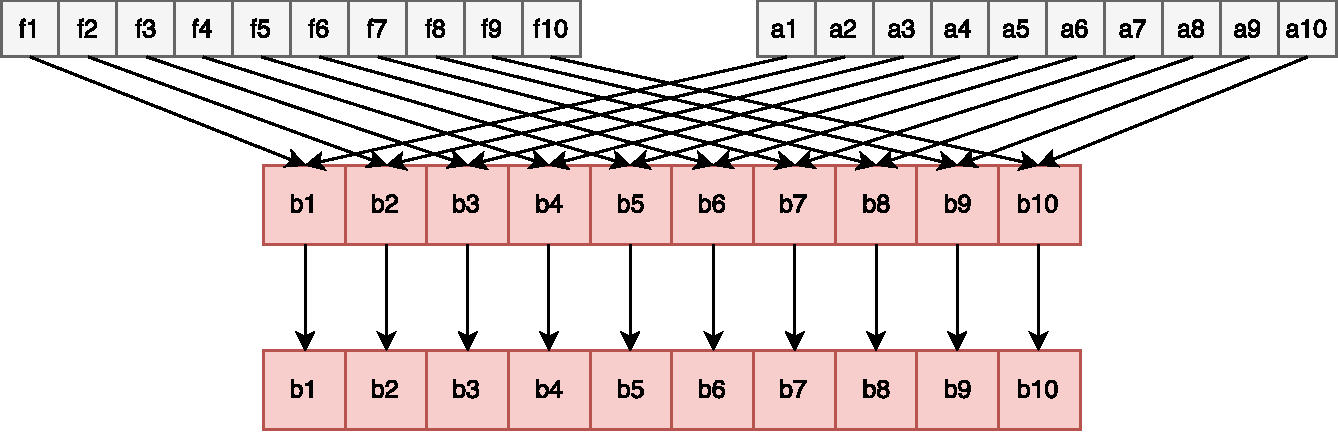
\includegraphics[scale=0.5]{images/parEvalNMulticore}
	\caption{Dataflow of the Multicore Haskell parEvalN version}
\end{figure} %$ %% formatting

\subsubsection{ParMonad}
The \inlinecode{Par} monad\footnote{It can be found in the \texttt{monad-par} package on hackage under \url{https://hackage.haskell.org/package/monad-par-0.3.4.8/}.} introduced by \citet{monad_par_paper_2011}, is a monad designed for composition of parallel programs.


Our parallel evaluation function \inlinecode{parEvalN} can be defined by zipping the list of \inlinecode{[a -> b]} with the list of inputs \inlinecode{[a]} with the application operator \inlinecode{\$} just like with Multicore Haskell. Then, we map over this not yet evaluated lazy list of results \inlinecode{[b]} with \inlinecode{spawnP :: NFData a => a -> Par (IVar a)} to transform them to a list of not yet evaluated forked away computations \inlinecode{[Par (IVar b)]}, which we convert to \inlinecode{Par [IVar b]} with \inlinecode{sequenceA}. We wait for the computations to finish by mapping over the \inlinecode{IVar b}'s inside the \inlinecode{Par} monad with \inlinecode{get}. This results in \inlinecode{Par [b]}. We finally execute this process with \inlinecode{runPar} to finally get \inlinecode{[b]} again.

\textbf{\textcolor{red}{explain problems with laziness here. Problems with torus}}

\begin{lstlisting}[frame=htrbl]
parEvalN :: (NFData b) => [a -> b] -> [a] -> [b]
parEvalN fs as = runPar $ 
	(sequenceA $ map (spawnP) $ zipWith ($) fs as) >>= mapM get
\end{lstlisting}
\begin{figure}[h]
	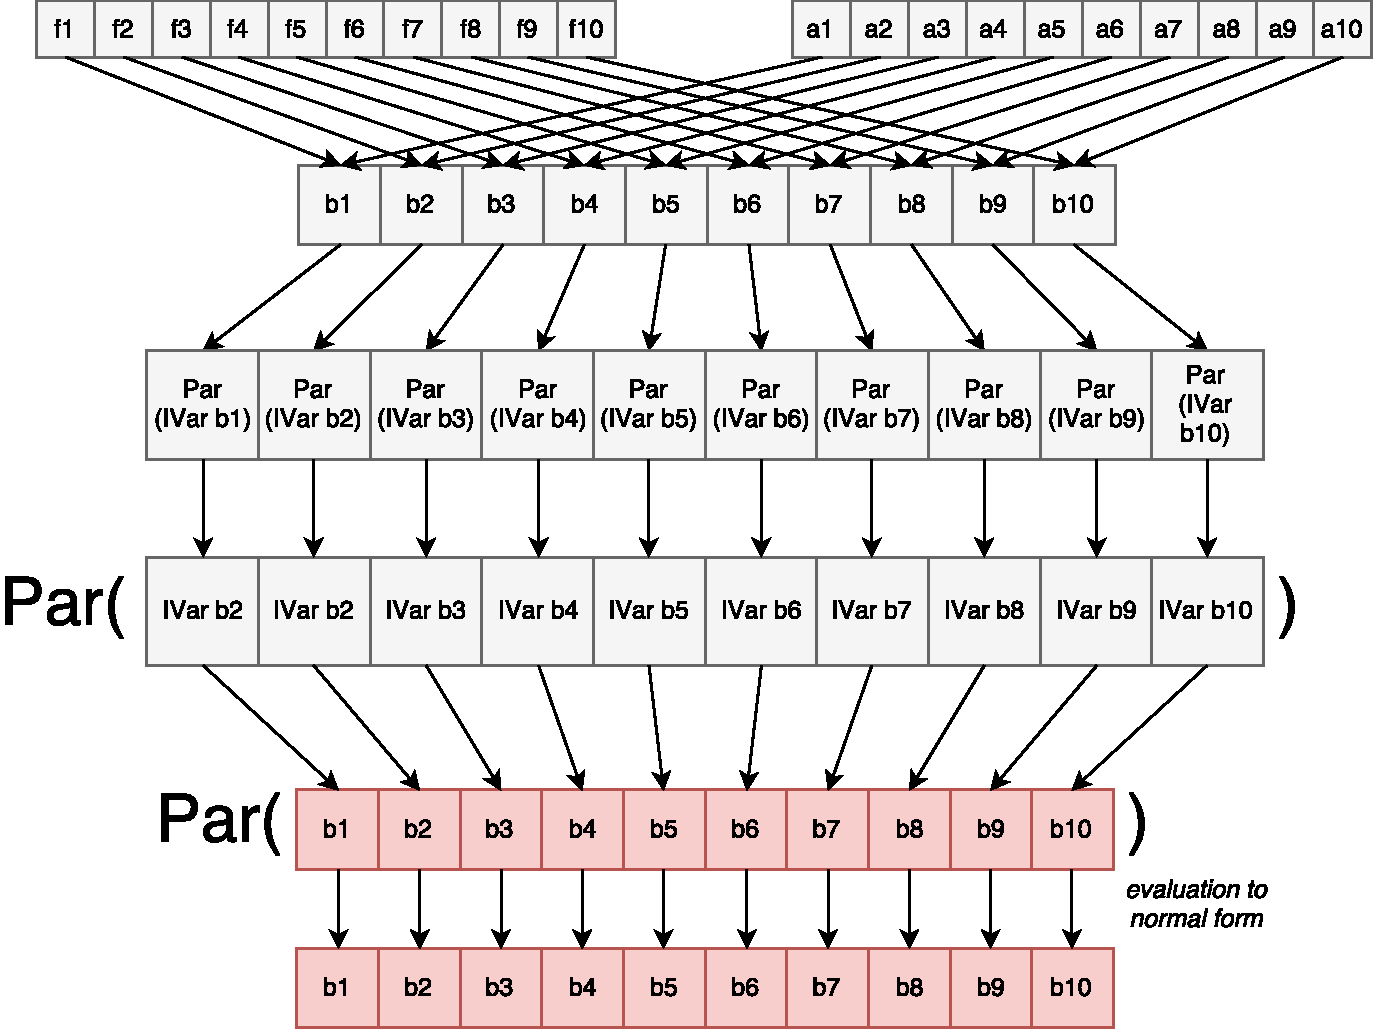
\includegraphics[scale=0.5]{images/parEvalNParMonad}
	\caption{Dataflow of the Par Monad parEvalN version}
\end{figure}

\subsubsection{Eden}
Eden \cite{eden,Loogen2012} is a parallel Haskell for distributed memory and comes with a MPI and a PVM backends.\footnote{See also \url{http://www.mathematik.uni-marburg.de/~eden/} and \url{https://hackage.haskell.org/package/edenmodules-1.2.0.0/}.} This means that it works on clusters as well so it makes sense to have a Eden-based backend for our new parallel Haskell flavour.

Eden was designed to work on clusters, but with a further simple backend it operates on multicores. However, in contrast to many other parallel Haskells, in Eden each process has its own heap. This seems to be a waste of memory, but with distributed programming paradigm and individual GC per process, Eden yields good performance results also on multicores \cite{arcs-dc,aswad2009low}.

While Eden also comes with a monad \inlinecode{PA} for parallel evaluation, it also ships with a completely functional interface that includes
%\\
%\inlinecode{spawnF :: (Trans a, Trans b) => [a -> b] -> [a] -> [b]}.
%\\
a \inlinecode{spawnF} function that
%This 
allows us to define \inlinecode{parEvalN} directly:

\begin{lstlisting}[frame=htrbl]
parEvalN :: (Trans a, Trans b) => [a -> b] -> [a] -> [b]
parEvalN = spawnF 
\end{lstlisting}
\begin{figure}[h]
	\includegraphics[scale=0.5]{images/parEvalNEden}
	\caption{Dataflow of the Eden parEvalN version}
\end{figure}

\paragraph{Eden TraceViewer.}
To comprehend the efficiency and the lack thereof in a parallel program, an inspection of its execution is extremely helpful. While some large-scale solutions exist \cite{Geimer2010}, the parallel Haskell community mainly utilises the tools Threadscope \cite{Wheeler2009} and Eden TraceViewer\footnote{See ..... on hackage for the last available version of Eden TraceViewer. There was an effort to implement the TraceViewer using modern web technologies \cite{traceviewer-web}.} \cite{Berthold2007a}. In the next sections we will present some \emph{traces}, the post-mortem process diagrams of Eden processes and their activity.

In a trace, the $x$ axis shows the time, the $y$ axis enumerates the machines and processes. A~trace shows a running process in green, a blocked process is red. If the process is \enquote{runnable}, \ie it may run, but does not, it is yellow. The typical reason for then is GC. An inactive machine where no processes are started yet, or all are already terminated, is shows as a blue bar. A~comminication from one process to another is represented with a black arrow. A~stream of communications, \eg a transmitted list is shows as a dark shading between sender and receiver processes.

\olcomment{show example trace or refer to a trace in later figures}


%%% Local Variables:
%%% mode: latex
%%% TeX-master: "main"
%%% End:
	\subsection{Arrows}
\label{sec:arrows}
\begin{figure}[h]
	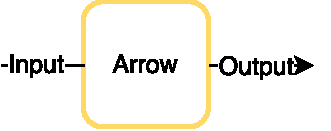
\includegraphics{images/arrow}
	\caption{Schematic depiction of an arrow}
\end{figure}
Arrows were introduced by \citet{HughesArrows} as a general interface for computation. An arrow \inlinecode{arr a b} represents  a computation that converts an input \inlinecode{a} to an output \inlinecode{b}. This is defined in the arrow typeclass:

\begin{figure}[h]
\begin{subfigure}{0.5\textwidth}
%\begin{minipage}{0.5\textwidth}
\begin{lstlisting}[frame=htrbl]
class Arrow arr where
arr :: (a -> b) -> arr a b



(>>>) :: arr a b -> arr b c -> arr a c




first :: arr a b -> arr (a,c) (b,c)
\end{lstlisting}
\caption{Arrow class definition}
%\end{minipage}
\end{subfigure}
~~~~
\begin{subfigure}{0.45\textwidth}
	\begin{center}
	\subcaptionbox{arr}{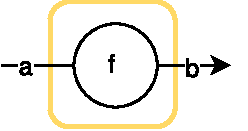
\includegraphics[scale=0.6]{images/arr}}
	\subcaptionbox{composition \inlinecode{(>>>)}}{\includegraphics[scale=0.6]{images/compose}}
	\subcaptionbox{first}{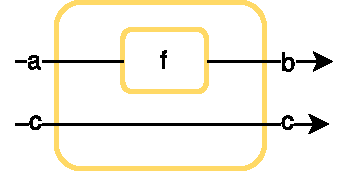
\includegraphics[scale=0.6]{images/first}}
	\end{center}
\end{subfigure}
\caption{The arrow type class definition on the left with schematic depiction of its combinators on the right}
\end{figure}
\lstinline{arr} is used to lift an ordinary function to an arrow type, similarly to the monadic \lstinline{return}. The \lstinline{>>>} operator is analogous to the monadic composition  \lstinline{>>=} and combines two arrows \inlinecode{arr a b} and \inlinecode{arr b c} by "wiring" the outputs of the first to the inputs to the second to get a new arrow \inlinecode{arr a c}. Lastly, the \lstinline{first} operator  takes the input arrow from \lstinline{b} to \lstinline{c} and converts it into an arrow on pairs with the second argument untouched. It allows us to to save input across arrows.
\\\\
The most prominent instances of this interface are regular functions \lstinline{(->)} (Fig.~\ref{fig:arrowfn}),
\begin{figure}[h]
\begin{lstlisting}[frame=htrbl]
instance Arrow (->) where
	arr f = f
	f >>> g = g . f
	first f = \(a, c) -> (f a, c) 
\end{lstlisting}
\caption{Arrow instance for regular functions}
\label{fig:arrowfn}
\end{figure}
and the Kleisli type (Fig.~\ref{fig:arrowkleisli}).
\begin{figure}[h]
\begin{lstlisting}[frame=htrbl]
data Kleisli m a b = Kleisli { run :: a -> m b }

instance Monad m => Arrow (Kleisli m) where
	arr f = Kleisli (return . f)
	f >>> g = Kleisli (\a -> f a >>= g)
	first f = Kleisli (\(a,c) -> f a >>= \b -> return (b,c))
\end{lstlisting}%$
\caption{Definition of the Kleisli type and the corresponding arrow instance}
\label{fig:arrowkleisli}
\end{figure}
\begin{figure}[h]
	\centering
	\begin{tabular}{cc}
		\subcaptionbox{first\label{t1}}{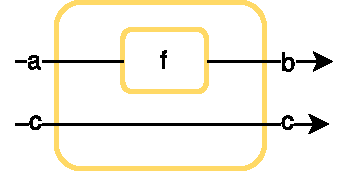
\includegraphics[width = 1.5in]{images/first}} &
		\subcaptionbox{second\label{fig:secondImg}}{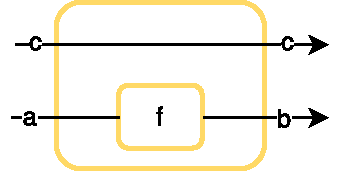
\includegraphics[width = 1.5in]{images/second}} \\
		\subcaptionbox{(***)\label{fig:***Img}}{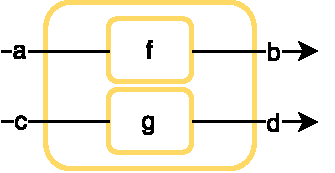
\includegraphics[width = 1.5in]{images/starstarstar}} &
		\subcaptionbox{(\&\&\&)\label{fig:&&&Img}}{\includegraphics[width = 1.5in]{images/andandand}}\
	\end{tabular}
	\caption{Syntactic sugar for arrows}
	\label{3}
\end{figure}
With this typeclass in place, Hughes also defined some syntactic sugar: The mirrored version of \inlinecode{first}, called \inlinecode{second} (Fig.~\ref{fig:secondImg},~\ref{fig:second}),
\begin{figure}[h]
\begin{lstlisting}[frame=htrbl]
second :: Arrow arr => arr a b -> arr (c, a) (c, b)
second f = arr swap >>> first f >>> arr swap
	where swap (x, y) = (y, x)
\end{lstlisting}
\caption{The second combinator}
\label{fig:second}
\end{figure}
the *** combinator which combines first and second to handle two inputs in one arrow, (Fig.\ref{fig:***Img},~\ref{fig:***})
\begin{figure}[h]
\begin{lstlisting}[frame=htrbl]
(***) :: Arrow arr => arr a b -> arr c d -> arr (a, c) (b, d)
f *** g = first f >>> second g
\end{lstlisting}
\caption{The (***) combinator}
\label{fig:***}
\end{figure}
and the \inlinecode{\&\&\&} combinator that constructs an arrow which outputs two different values like \inlinecode{***}, but takes only one input (Fig.~\ref{fig:&&&Img},~\ref{fig:&&&}).
\begin{figure}[h]
\begin{lstlisting}[frame=htrbl]
(&&&) :: Arrow arr => arr a b -> arr a c -> a a (b, c)
f &&& g = arr (\a -> (a, a)) >>> (f *** g)
\end{lstlisting}
\caption{The (\&\&\&) combinator}
\label{fig:&&&}
\end{figure}
A short example given by Hughes on how to use this is \lstinline{add} over arrows, which can be seen in Fig.~\ref{fig:addArrows}.
\begin{figure}[h]
\begin{lstlisting}[frame=htrbl]
add :: Arrow arr => arr a Int -> arr a Int -> arr a Int
add f g = (f &&& g) >>> arr (\(u, v) -> u + v)
\end{lstlisting}
\caption{Add over arrows}
\label{fig:addArrows}
\end{figure}
% The benefit of using the \inlinecode{Arrow} typeclass is that any type which is shown to be an arrow can be used in conjunction with this newly created \lstinline{add} combinator. Even though this example is quite simple, the power of the arrow interface immediately is clear: If a type is an arrow, it can automatically used together with every library that works on arrows. Compared to simple monads, this enables us to write code that is more extensible, without touching the internals of the specific arrows.
% \\\\
% \textit{Note: In the definitions Hughes gave in his paper, the notation \inlinecode{a b c} for an arrow from \inlinecode{b} to \inlinecode{c} is used. We use the equivalent definition \inlinecode{arr a b} for an arrow from \inlinecode{a} to \inlinecode{b} instead, to make it easier to find the arrow type in type signatures.}
%

The more restrictive interface of arrows (a monad can be \emph{anything}, an arrow is a process of doing something, a \emph{computation}) allows for more elaborate composition and transformation combinators. One of the major problems in parallel computing is composition of parallel processes.


%%% Local Variables:
%%% mode: latex
%%% TeX-master: "main"
%%% End:
	%\pagebreak
	\section{Related Work}
\label{sec:related-work}

\olcomment{arrows or Arrows?}

\subsection{Parallel Haskells}
Of course, the three parallel Haskell flavours we have presented above: the GpH \cite{Trinder1998a,Trinder1999} parallel Haskell dialect and its multicore version \cite{Marlow2009}, the \inlinecode{Par} monad \cite{par-monad,Foltzer:2012:MPC:2398856.2364562}, and Eden \cite{eden,Loogen2012} are related to this work. We use these languages as backends: our library can switch from one to other at user's command.

HdpH \cite{Maier:2014:HDS:2775050.2633363,stewart_maier_trinder_2016} is an extension of \inlinecode{Par} monad to heterogeneous clusters. LVish \cite{Kuper:2014:TPE:2666356.2594312} is a communication-centred extension of \inlinecode{Par} monad.
%
Further parallel Haskell approaches include pH \cite{ph-book}, research work done on distributed variants of GpH \cite{Trinder1996,Aljabri:2013:DIG:2620678.2620682,Aljabri2015} and low-level Eden implementation \cite{JostThesis,berthold_loidl_hammond_2016}. Skeleton composition \cite{dieterle_horstmeyer_loogen_berthold_2016}, communication \cite{Dieterle2010}, and generation of process networks \cite{Horstmeyer2013} are recent in-focus research topics in Eden. This also includes the definitions of new skeletons \cite{doi:10.1142/S0129626403001380,Eden:PARCO05,Berthold2009-mr,Berthold2009-fft,brown2010ever,dieterle2010skeleton,delaEncina2011,Dieterle2013}.

More different approaches include data parallelism \cite{Chakravarty2007,Keller:2010:RSP:1932681.1863582,}, GPU-based approaches \cite{Mainland:2010:NEC:2088456.1863533,obsidian-phd}, software transactional memory \cite{Harris:2005:CMT:1065944.1065952,Perfumo:2008:LST:1366230.1366241}.
%
The Haskell--GPU bridge Accelerate \cite{Chakravarty:2011:AHA:1926354.1926358,CMCK14,McDonell:2015:TRC:2887747.2804313} deserves a special mention. Accelerate is completely orthogonal to our approach. \citeauthor{marlow2013parallel} authored a recent book \citeyear{marlow2013parallel} on parallel Haskells.

\subsection{Algorithmic skeletons}

Algorithmic skeletons were introduced by \citet{Cole1989}.
Early efforts include \cite{darlington1993parallel,botorog1996efficient,p3l97,Gorlatch1998,Lengauer1997}. \citet{SkeletonBook} consolidated early reports on high-level programming approaches.
The effort is ongoing, including topological skeletons \cite{Eden:PARCO05}, special-purpose skeletons for computer algebra \cite{Berthold2009-fft,brown2010ever,lobachev-phd,Lobachev2012}, iteration skeletons \cite{Dieterle2013}. The idea of \citet{scscp} is to use a parallel Haskell to orchestrate further software systems to run in parallel. \citet{dieterle_horstmeyer_loogen_berthold_2016} compare the composition of skeleton to stable process networks.

\subsection{Arrows}

Arrows were introduced by \citet{HughesArrows}, basically they are a generalised function arrow~\inlinecode{->}. \citet{Hughes2005} is a tutorial on arrows. Some theoretical details on arrows \cite{jacobs_heunen_hasuo_2009,LINDLEY201197,ATKEY201119} are viable. \citet{Paterson:2001:NNA:507669.507664} introduced a new notation for arrows. Arrows have applications in information flow research \cite{1648705,LI20101974,Russo:2008:LLI:1411286.1411289}, invertible programming \cite{Alimarine:2005:BAA:1088348.1088357}, and quantum computer simulation \cite{vizzotto_altenkirch_sabry_2006}. But perhaps most prominent application of arrows is functional reactive programming \cite{Hudak2003}.\olcomment{cite more!}

\citet{Liu:2009:CCA:1631687.1596559} formally define a more special kind of arrows that capsule the computation more than regular arrows do and thus enable optimizations. Their approach would allow parallel composition, as their special arrows would not interfere with each other in concurrent execution. In a contrast, we capture a whole parallel computation as a single entity: our main instantiation function \inlinecode{parEvalN} makes a single (parallel) arrow out of list of arrows.\olcomment{ugh, take care!}
\citet{Huang2007} utilise arrows for parallelism, but strikingly different from our approach. They basically use arrows to orchestrate several tasks in robotics. We propose a general interface for parallel programming, remaining completely in Haskell.

\subsection{Other languages}

Although this work is centred on Haskell implementation of arrows, it is applicable to any functional programming language where parallel evaluation and arrows can be defined. Our experiments with our approach in Frege language (which is basically Haskell on the JVM) were quite successful, we were able to use typical Java libraries for parallelism. However, it is beyond the scope of this work.

\citet{achten2004arrows,achten2007arrow} use an arrow implementation in Clean for better handling of typical GUI tasks. \citet{Dagand:2009:ORD:1481861.1481870} used arrows in OCaml in the implementation of a distributed system.


%%% Local Variables:
%%% mode: latex
%%% TeX-master: "main"
%%% End:
	%\pagebreak
	%\pagebreak
	\section{Parallel Arrows}
\label{sec:parallel-arrows}
We have seen what Arrows are and how they can be used as a general interface to computation. In the following section we will discuss how Arrows constitute a general interface not only to computation, but to \textbf{parallel computation} as well. We start by introducing the interface and explaining the reasonings behind it. Then, we discuss some implementations using exisiting parallel Haskells. Finally, we explain why using Arrows for expressing parallelism is beneficial.
\subsection{The ArrowParallel typeclass}
As we have seen earlier, in its purest form, parallel computation (on functions) can be seen as the execution of some functions \inlinecode{a -> b} in parallel, \inlinecode{parEvalN} (Fig.~\ref{fig:parEvalNTypeSig},~\ref{fig:parEvalN}).
Translating this into arrow terms gives us a new operator \inlinecode{parEvalN} that lifts a list of arrows \inlinecode{[arr a b]} to a parallel arrow \inlinecode{arr [a] [b]} (Fig.~\ref{fig:parEvalNArrowFn}) (This combinator is similar to our utility function \lstinline{listApp} from Appendix \ref{utilfns}, but does parallel instead of serial evaluation).
\begin{figure}[h]
\begin{lstlisting}[frame=htrbl]
parEvalN :: (Arrow arr) => [arr a b] -> arr [a] [b]
\end{lstlisting}
\caption{parEvalN Arrow combinator as a function}
\label{fig:parEvalNArrowFn}
\end{figure}
With this definition of \inlinecode{parEvalN}, parallel execution is yet another arrow combinator. But as the implementation may differ depending on the actual type of the arrow \inlinecode{arr} and we want this to be an interface for different backends, we introduce a new typeclass \inlinecode{ArrowParallel arr a b} to host this combinator (Fig.~\ref{fig:parEvalNArrowTypeClass1}).
\begin{figure}[h]
\begin{lstlisting}[frame=htrbl]
class Arrow arr => ArrowParallel arr a b where
	parEvalN :: [arr a b] -> arr [a] [b]
\end{lstlisting}
\caption{parEvalN Arrow combinator in a first version of the ArrowParallel typeclass}
\label{fig:parEvalNArrowTypeClass1}
\end{figure}
Sometimes parallel Haskells require or allow for additional configuration parameters, \eg an information about the execution environment or the level of evaluation (weak-head normalform vs. normalform). For this reason we also introduce an additional \inlinecode{conf} parameter to the function. We also do not want \inlinecode{conf} to be a fixed type, as the configuration parameters can differ for different instances of \inlinecode{ArrowParallel}. So we add it to the type signature of the typeclass as well and get \inlinecode{ArrowParallel arr a b conf} (Fig.~\ref{fig:parEvalNArrowTypeClassFinal}).
\begin{figure}[h]
\begin{lstlisting}[frame=htrbl]
class Arrow arr => ArrowParallel arr a b conf where
	parEvalN :: conf -> [arr a b] -> arr [a] [b]
\end{lstlisting}
\caption{parEvalN Arrow combinator in the final version of the ArrowParallel typeclass}
\label{fig:parEvalNArrowTypeClassFinal}
\end{figure}
Note that we don't require the \inlinecode{conf} parameter in every implementation. If it is not needed, we usually just default the \inlinecode{conf} type parameter to () and even blank it out in the parameter list of the implemented \inlinecode{parEvalN}, as we will see in the implementation of the Multicore and the ParMonad backend.

\subsection{ArrowParallel instances}

\subsubsection{Multicore Haskell} \label{sec:parrows:multicore}
The Multicore Haskell implementation of this class is implemented in a straightforward manner by using listApp from appendix \ref{utilfns} combined with the \inlinecode{withStrategy :: Strategy a -> a -> a} and \inlinecode{pseq :: a -> b -> b} combinators from Multicore Haskell, where \inlinecode{withStrategy} is the same as \inlinecode{using :: a -> Strategy a -> a} but with flipped parameters.
\begin{figure}[h]
\begin{lstlisting}[frame=htrbl]
instance (NFData b, ArrowApply arr, ArrowChoice arr) =>
	ArrowParallel arr a b () where
    	parEvalN _ fs =
       		listApp fs >>>
        	arr (withStrategy (parList rdeepseq)) &&& arr id >>>
        	arr (uncurry pseq)
\end{lstlisting}% $ %% formatting
\caption{Fully evaluating ArrowParallel instance for the Multicore Haskell backend}
\label{fig:ArrowParallelMulticoreRdeepseq}
\end{figure}
For most cases a fully evaluating version like in Fig.~\ref{fig:ArrowParallelMulticoreRdeepseq} would probably suffice, but as the Multicore Haskell interface allows the user to specify the level of evaluation to be done via the \inlinecode{Strategy} interface, we want to the user not to lose this ability because of using our API. We therefore introduce the \inlinecode{Conf a} data-type that simply wraps a \inlinecode{Strategy a} (Fig.~\ref{fig:confa}). We can't directly use the \inlinecode{Strategy a} type here as GHC (at least in the versions used for development in this paper) does not allow type synonyms in type class instances.
\begin{figure}[h]
\begin{lstlisting}[frame=htrbl]
data Conf a = Conf (Strategy a)
\end{lstlisting}
\caption{Definition of Conf a}
\label{fig:confa}
\end{figure}
To get our configurable \inlinecode{ArrowParallel} instance, we simply unwrap the strategy and pass it to \inlinecode{parList} like in the fully evaluating version (Fig.~\ref{fig:ArrowParallelMulticoreConfigurable}).
\begin{figure}[h]
\begin{lstlisting}[frame=htrbl]
instance (NFData b, ArrowApply arr, ArrowChoice arr) =>
	ArrowParallel arr a b (Conf b) where
    	parEvalN (Conf strat) fs =
        	listApp fs >>>
        	arr (withStrategy (parList strat)) &&& arr id >>>
        	arr (uncurry pseq)
\end{lstlisting}
\caption{Configurable ArrowParallel instance for the Multicore Haskell backend}
\label{fig:ArrowParallelMulticoreConfigurable}
\end{figure}
\subsubsection{Par Monad}
The ParMonad implementation (Fig.~\ref{fig:ArrowParallelParMonad}) makes use of Haskells laziness and ParMonad's \inlinecode{spawnP :: NFData a =>\ \ a -> Par (IVar a)} function. The latter forks away the computation of a value and returns an \inlinecode{IVar} containing the result in the \inlinecode{Par} monad.


We therefore apply each function to its corresponding input value with \inlinecode{listApp} (Fig.~\ref{fig:listApp}) and then fork the computation away with \inlinecode{arr spawnP} inside a \inlinecode{zipWithArr} call. This yields a list \inlinecode{[Par (IVar b)]}, which we then convert into \inlinecode{Par [IVar b]} with \inlinecode{arr sequenceA}. In order to wait for the computation to finish, we map over the \inlinecode{IVar}s inside the ParMonad with \inlinecode{arr (>>= mapM get)}. The result of this operation is a \inlinecode{Par [b]} from which we can finally remove the monad again by running \inlinecode{arr runPar} to get our output of \inlinecode{[b]}.
\begin{figure}[h]
\begin{lstlisting}[frame=htrbl]
instance (NFData b, ArrowApply arr, ArrowChoice arr) =>
	ArrowParallel arr a b conf where
		parEvalN _ fs = 
			(arr $ \as -> (fs, as)) >>>
			zipWithArr (app >>> arr spawnP) >>>
			arr sequenceA >>>
			arr (>>= mapM get) >>>
			arr runPar
\end{lstlisting} %$ %% formatting
\caption{ArrowParallel instance for the Par Monad backend}
\label{fig:ArrowParallelParMonad}
\end{figure}

\subsubsection{Eden}
For the Multicore and ParMonad implementation we could use general instances of \inlinecode{ArrowParallel} that just require the \inlinecode{ArrowApply} and \inlinecode{ArrowChoice} typeclasses. With Eden this is not the case as we can only spawn a list of functions and we cannot extract simple functions out of arrows. While we could still manage to have only one class in the module by introducing a typeclass \inlinecode{ArrowUnwrap} (Fig.~\ref{fig:ArrowUnwrap}).
\begin{figure}[h]
\begin{lstlisting}[frame=htrbl]
class (Arrow arr) => ArrowUnwrap arr where
	arr a b -> (a -> b)
\end{lstlisting}
\caption{possible ArrowUnwrap typeclass}
\label{fig:ArrowUnwrap}
\end{figure}
We don't do it here for aesthetic resons, though. For now, we just implement \inlinecode{ArrowParallel} for normal functions (Fig.~\ref{fig:ArrowParallelEdenFns})
\begin{figure}[h]
\begin{lstlisting}[frame=htrbl]
instance (Trans a, Trans b) => ArrowParallel (->) a b conf where
parEvalN _ fs as = spawnF fs as
\end{lstlisting}
\caption{ArrowParallel instance for functions in the Eden backend}
\label{fig:ArrowParallelEdenFns}
\end{figure}
and the Kleisli type (Fig.~\ref{fig:ArrowParallelEdenKleisli}).
\begin{figure}[h]
\begin{lstlisting}[frame=htrbl]
instance (Monad m, Trans a, Trans b, Trans (m b)) =>
	ArrowParallel (Kleisli m) a b conf where
parEvalN conf fs =
	(arr $ parEvalN conf (map (\(Kleisli f) -> f) fs)) >>>
	(Kleisli $ sequence)
\end{lstlisting}
\caption{ArrowParallel instance for the Kleisli type in the Eden backend}
\label{fig:ArrowParallelEdenKleisli}
\end{figure}

\FloatBarrier

\subsection{Impact of parallel Arrows}
\olcomment{move this to Contributions in the front or something}
We have seen that we can wrap parallel Haskells inside of the \inlinecode{ArrowParallel} interface, but why do we abstract parallelism this way and what does this approach do better than the other parallel Haskells?
\begin{itemize}
	\item \textbf{Arrow API benefits}:
	With the \inlinecode{ArrowParallel} typeclass we do not lose any benefits of using arrows as \inlinecode{parEvalN} is just yet another arrow combinator. The resulting arrow can be used in the same way a potential serial version could be used. This is a big advantage of this approach, especially compared to the monad solutions as we do not introduce any new types. We can just \enquote{plug} in parallel parts into our sequential programs without having to change anything.
	\item \textbf{Abstraction}:
	With the \inlinecode{ArrowParallel} typeclass, we abstracted all parallel implementation logic away from the business logic. This gives us the beautiful situation of being able to write our code against the interface the typeclass gives us without being bound to any parallel Haskell. So as an example, during development, we can run the code on the simple Multicore version and afterwards deploy it on a cluster by converting it into an Eden version, by just replacing the actual \inlinecode{ArrowParallel} instance.
\end{itemize}


%%% Local Variables:
%%% mode: latex
%%% TeX-master: "main"
%%% End:
	%\pagebreak
	\subsection{Extending the Interface}
\label{sec:extending-interface}
With the \inlinecode{ArrowParallel} typeclass in place and implemented, we can now implement some further basic parallel interface functions. These are algorithmic skeletons that, however, mostly serve as a foundation to further, more specific algorithmic skeletons.

\subsubsection{Lazy \inlinecode{parEvalN}}
\begin{figure}[h]
	\includegraphics[scale=0.7]{images/parEvalNLazy}
	\caption{Schematic depiction of parEvalNLazy}
	\label{fig:parEvalNLazyImg}
\end{figure}
The function \inlinecode{parEvalN} is 100\% strict, which means that it fully evaluates all passed arrows. Sometimes this might not be feasible, as it will not work on infinite lists of functions like e.g. \inlinecode{map (arr . (+)) [1..]} or just because we need the arrows evaluated in chunks. \inlinecode{parEvalNLazy} (Fig.~\ref{fig:parEvalNLazyImg},~\ref{fig:parEvalNLazy}) fixes this. It works by first chunking the input from \inlinecode{[a]} to \inlinecode{[[a]]} with the given \inlinecode{ChunkSize} in \inlinecode{arr (chunksOf chunkSize)}. These chunks are then fed into a list \inlinecode{[arr [a] [b]]} of parallel arrows created by feeding chunks of the passed \inlinecode{ChunkSize} into the regular parEvalN by using \inlinecode{listApp} (Fig.~\ref{fig:listApp}). The resulting \inlinecode{[[b]]} is lastly converted into \inlinecode{[b]} with \inlinecode{arr concat}.
\begin{figure}[h]
\begin{lstlisting}[frame=htrbl]
parEvalNLazy :: (ArrowParallel arr a b conf, ArrowChoice arr, ArrowApply arr) =>
	conf -> ChunkSize -> [arr a b] -> (arr [a] [b])
parEvalNLazy conf chunkSize fs =
	arr (chunksOf chunkSize) >>>
	listApp fchunks >>>
	arr concat
	where fchunks = map (parEvalN conf) $ chunksOf chunkSize fs
\end{lstlisting} %$ %% formatting
\caption{Definition of parEvalNLazy}
\label{fig:parEvalNLazy}
\end{figure}

\subsubsection{Heterogenous tasks}
\begin{figure}[h]
	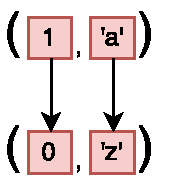
\includegraphics[scale=0.7]{images/parEval2}
	\caption{Schematic depiction of parEval2}
	\label{fig:parEval2Img}
\end{figure}
We have only talked about the paralellization arrows of the same type until now. But sometimes we want to paralellize heterogenous types as well. However, we can implement such a \inlinecode{parEval2} combinator (Fig.~\ref{fig:parEval2Img},~\ref{fig:parEval2}) which combines two arrows \inlinecode{arr a b} and \inlinecode{arr c d} into a new parallel arrow \inlinecode{arr (a, c) (b, d)} quite easily with the help of the \inlinecode{ArrowChoice} typeclass. The idea is to use the \inlinecode{+++} combinator which combines two arrows \inlinecode{arr a b} and \inlinecode{arr c d} and transforms them into \inlinecode{arr (Either a c) (Either b d)} to get a common arrow type that we can then feed into parEvalN.
\\\\
We start by transforming the \inlinecode{(a, c)} input into a 2-element list \inlinecode{[Either a c]} by first tagging the two inputs with \inlinecode{Left} and \inlinecode{Right} and wrapping the right element in a singleton list with \inlinecode{return} so that we can combine them with \inlinecode{arr (uncurry (:))}. Next, we feed this list into a parallel arrow running on 2 instances of \inlinecode{f +++ g} as described above. After the calculation is finished, we convert the resulting \inlinecode{[Either b d]} into \inlinecode{([b], [d])} with \inlinecode{arr partitionEithers}. The two lists in this tuple contain only 1 element each by construction, so we can finally just convert the tuple to \inlinecode{(b, d)} in the last step.
\begin{figure}[h]
\begin{lstlisting}[frame=htrbl]
parEval2 :: (ArrowChoice arr,
	ArrowParallel arr (Either a c) (Either b d) conf) =>
	conf -> arr a b -> arr c d -> arr (a, c) (b, d)
parEval2 conf f g =
	arr Left *** (arr Right >>> arr return) >>>
	arr (uncurry (:)) >>>
	parEvalN conf (replicate 2 (f +++ g)) >>>
	arr partitionEithers >>>
	arr head *** arr head
\end{lstlisting}
	\caption{Definition of parEval2}
	\label{fig:parEval2}
\end{figure}


%%% Local Variables:
%%% mode: latex
%%% TeX-master: "main"
%%% End:
	%\pagebreak
	\subsubsection{Syntactic Sugar} \label{syntacticSugar}
For basic arrows, we have the \inlinecode{(***)} combinator (Fig.~\ref{fig:***Img},~\ref{fig:***}) which allows us to combine two arrows \inlinecode{arr a b} and \inlinecode{arr c d} into an arrow \inlinecode{arr (a, c) (b, d)} which does both computations at once. This can easily be translated into a parallel version \inlinecode{(\ensuremath{\mathbin{***}})} (Fig.~\ref{fig:par***}) with the use of \inlinecode{parEval2}, but for this we require a backend which has an implementation that does not require any configuration (hence the \inlinecode{()} as the conf parameter in Fig.~\ref{fig:par***}).
\begin{figure}[h]
\begin{lstlisting}[frame=htrbl]
(\ensuremath{\mathbin{***}}) :: (ArrowChoice arr, ArrowParallel arr (Either a c) (Either b d) ())) =>
	arr a b -> arr c d -> arr (a, c) (b, d)
(\ensuremath{\mathbin{***}}) = parEval2 ()
\end{lstlisting}
\caption{Definition of (\ensuremath{\mathbin{***}}) - the parallel version of (***)}
\label{fig:par***}
\end{figure}
% With this we can analogously to the serial \inlinecode{&&&}
We define the parallel \inlinecode{(\ensuremath{\mathbin{\char92 \&\char92 \&\char92 \&}})} (Fig.~\ref{fig:par&&&}) in a similar manner to its sequential pendant \inlinecode{(\&\&\&)} (Fig.~\ref{fig:&&&Img},~\ref{fig:&&&}).
\begin{figure}[h]
\begin{lstlisting}[frame=htrbl]
(\ensuremath{\mathbin{\&\&\&}}) :: (ArrowChoice arr, ArrowParallel arr (Either a a) (Either b c) ()) =>
	arr a b -> arr a c -> arr a (b, c)
(\ensuremath{\mathbin{\&\&\&}}) f g = (arr $ \a -> (a, a)) >>> f \ensuremath{\mathbin{***}} g
\end{lstlisting} % $ %% formatting
\caption{Definition of (\ensuremath{\mathbin{\char92 \&\char92 \&\char92 \&}}) - the parallel version of (\&\&\&)}
\label{fig:par&&&}
\end{figure}
	%\pagebreak
	\section{Futures} \label{futures}
Consider the parallel arrow combinator in Fig.~\ref{fig:someCombinator}
\begin{figure}[h]
\begin{lstlisting}[frame=htrbl]
someCombinator :: (Arrow arr) => [arr a b] -> [arr b c] -> arr [a] [c]
someCombinator fs1 fs2 = parEvalN () fs1 >>> rightRotate >>> parEvalN () fs2
\end{lstlisting}
\caption{An example parallel Arrow combinator without Futures}
\label{fig:someCombinator}
\end{figure}
In a distributed environment, the resulting arrow of this combinator first evaluates all \inlinecode{[arr a b]} in parallel, sends the results back to the master node, rotates the input once and then evaluates the \inlinecode{[arr b c]} in parallel to then gather the input once again on the master node.
Such situations arise, \eg in scientific computations when the data distributed across the nodes needs to be transposed. A concrete example is 2D FFT computation \cite{Gorlatch,Berthold2009-fft}.

While the example in Fig.~\ref{fig:someCombinator} could be rewritten into only one \inlinecode{parEvalN} call by directly wiring the arrows properly together, this example illustrates an important problem: When using a \inlinecode{ArrowParallel} backend that resides on multiple computers, all communication between the nodes is done via the master node, as shown in the Eden trace in Figure~\ref{fig:withoutFutures}. This can become a serious bottleneck %in heavy threaded applications.
for larger amount of data and number of processes \citep[showcases][as, \eg]{Berthold2009-fft}.
\begin{figure}[ht]
	\centering
	\includegraphics[width=0.9\textwidth]{images/withoutFutures}
	\caption[without Futures]{Communication between 4 threads without Futures. All communication goes through the master node. Each bar represents one process. Black lines between processes represent communication. Colors: blue $\hat{=}$ idle, green $\hat{=}$ running, red  $\hat{=}$ blocked, yellow $\hat{=}$ suspended.}
	\label{fig:withoutFutures}
\end{figure}

This motivates for an approach that allows the nodes to communicate directly with each other. Thankfully, Eden, the distributed parallel Haskell we have used in this paper so far, already ships with the concept of \inlinecode{RD} (remote data) that enables this behaviour \cite{AlGo03a,Dieterle2010}.

But as we want code written against our API to be implementation agnostic, we have to wrap this context. We do this with the \inlinecode{Future} typeclass (Fig.~\ref{fig:future}).
\begin{figure}[h]
\begin{lstlisting}[frame=htrbl]
class Future fut a \text{\tt \char124{}} a -> fut where
    put :: (Arrow arr) => arr a (fut a)
    get :: (Arrow arr) => arr (fut a) a
\end{lstlisting}
\caption{Definition of the Future typeclass}
\label{fig:future}
\end{figure}
Since \inlinecode{RD} is only a type synonym for communication type that Eden uses internally, we have to use some wrapper classes to fit that definition, though, as seen in Fig.~\ref{fig:RDFuture} (this is due to the same reason we had to introduce a wrapper for \inlinecode{Strategy a} in the Multicore Haskell implementation of \inlinecode{ArrowParallel} in chapter \ref{sec:parrows:multicore}).
\begin{figure}[h]
\begin{lstlisting}[frame=htrbl]
data RemoteData a = RD { rd :: RD a }

instance (Trans a) => Future RemoteData a where
    put = arr (\a -> RD { rd = release a })
    get = arr rd >>> arr fetch
\end{lstlisting}
\caption{RD based RemoteData version of Future for the Eden backend}
\label{fig:RDFuture}
\end{figure}

For our Par Monad and Multicore Haskell backends, we can simply use \inlinecode{MVar}s \cite{jones1996concurrent} (Fig.~\ref{fig:MVarFuture}), because we have shared memory in a single node and don't require Eden's sophisticated communication channels. \fixme{explain MVars}
\begin{figure}[h]
\begin{lstlisting}[frame=htrbl]
{-# NOINLINE putUnsafe #-}
putUnsafe :: a -> MVar a
putUnsafe a = unsafePerformIO $ do
    mVar <- newEmptyMVar
    putMVar mVar a
    return mVar

instance (NFData a) => Future MVar a where
    put = arr putUnsafe
    get = arr takeMVar >>> arr unsafePerformIO
\end{lstlisting}
\caption{MVar instance of the Future typeclass for the Par Monad and Multicore Haskell backends}
\label{fig:MVarFuture}
\end{figure}

Furthermore, in order for these \inlinecode{Future} types to fit with the \inlinecode{ArrowParallel} instances we gave earlier, we have to give the necessary \inlinecode{NFData} and \inlinecode{Trans} instances - the latter only being needed in Eden. Because \inlinecode{MVar} already ships with a \inlinecode{NFData} instance, we only have to supply two simple instances for our \inlinecode{RemoteData} type.
\begin{figure}[h]
\begin{lstlisting}[frame=htrbl]
instance NFData (RemoteData a) where
    rnf = rnf . rd
instance Trans (RemoteData a)
\end{lstlisting}
\caption{NFData and Trans instances for the RemoteData type. The Trans instance does not have any functions declared as the default implementation suffices here. See \url{https://hackage.haskell.org/package/edenmodules-1.2.0.0/docs/Control-Parallel-Eden.html\#g:5} for more information.}
\end{figure}

Going back to our communication example we can use this Future concept in order to enable direct communications between the nodes in the following way:
\begin{figure}[h]
\begin{lstlisting}[frame=htrbl]
someCombinator :: (Arrow arr) => [arr a b] -> [arr b c] -> arr [a] [c]
someCombinator fs1 fs2 =
	parEvalN () (map (>>> put) fs1) >>>
	rightRotate >>>
	parEvalN () (map (get >>>) fs2)
\end{lstlisting}
\caption{The combinator from Fig.~\ref{fig:someCombinator} in parallel}
\label{fig:someCombinatorParallel}
\end{figure}
In a distributed environment, this gives us a communication scheme with messages going through the master node only if it is needed - similar to what is shown in the trace in Fig.~\ref{fig:withFutures}.\olcomment{Fig.~3 is not really clear. Do Figs 2-3 with a lot of load?}
\begin{figure}[ht]
	\centering
	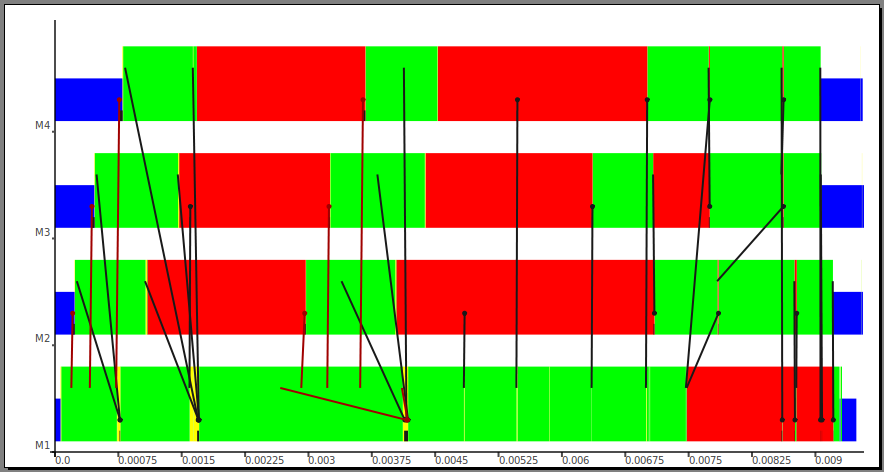
\includegraphics[width=0.9\textwidth]{images/withFutures}
	\caption[with Futures]{Communication between 4 threads with Futures. Other than in Fig.~\ref{fig:withoutFutures}, threads communicate directly (black lines between the bars) instead of always going through the master node (bottom bar).}
	\label{fig:withFutures}
\end{figure}
	%\pagebreak
	
\FloatBarrier
\section{Map-based Skeletons}
\label{sec:map-skeletons}
Now we have developed Parallel Arrows far enough to define some algorithmic skeletons useful to an application programmer.
\subsection{Parallel map}
\begin{figure}[h]
	\includegraphics[scale=0.7]{images/parMap}
	\caption{Schematic depiction of parMap}
	\label{fig:parMapImg}
\end{figure}
\inlinecode{parMap} (Fig.~\ref{fig:parMapImg},~\ref{fig:parMap}) is probably the most common skeleton for parallel programs. We can implement it with \inlinecode{ArrowParallel} by repeating an arrow \inlinecode{arr a b} and then passing it into \inlinecode{parEvalN} to get an arrow \inlinecode{arr [a] [b]}.
Just like \inlinecode{parEvalN}, \inlinecode{parMap} is 100 \% strict.
\begin{figure}[h]
\begin{lstlisting}[frame=htrbl]
parMap :: (ArrowParallel arr a b conf) =>
	conf -> (arr a b) -> (arr [a] [b])
parMap conf f = parEvalN conf (repeat f)
\end{lstlisting}
\caption{Definition of parMap}
\label{fig:parMap}
\end{figure}

\subsection{Lazy parallel map}
\begin{figure}[h]
	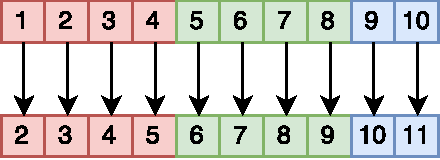
\includegraphics[scale=0.7]{images/parMapStream}
	\caption{Schematic depiction of parMapStream}
	\label{fig:parMapStreamImg}
\end{figure}
As \inlinecode{parMap} (Fig.~\ref{fig:parMapImg},~\ref{fig:parMap}) is 100\% strict it has the same restrictions as \inlinecode{parEvalN} compared to \inlinecode{parEvalNLazy}. So it makes sense to also have a \inlinecode{parMapStream} (Fig.~\ref{fig:parMapStreamImg},~\ref{fig:parMapStream}) which behaves like \inlinecode{parMap}, but uses \inlinecode{parEvalNLazy} instead of \inlinecode{parEvalN}.
\begin{figure}[h]
\begin{lstlisting}[frame=htrbl]
parMapStream :: (ArrowParallel arr a b conf, ArrowChoice arr, ArrowApply arr) =>
	conf -> ChunkSize -> arr a b -> arr [a] [b]
parMapStream conf chunkSize f = parEvalNLazy conf chunkSize (repeat f)
\end{lstlisting}
\caption{Definition of parMapStream}
\label{fig:parMapStream}
\end{figure}

\subsection{Statically load-balancing parallel map}
\begin{figure}[h]
	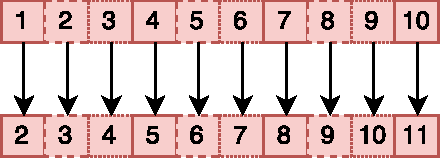
\includegraphics[scale=0.7]{images/farm}
	\caption{Schematic depiction of farm}
	\label{fig:farmImg}
\end{figure}
A \inlinecode{parMap} (Fig.~\ref{fig:parMapImg},~\ref{fig:parMap}) spawns every single computation in a new thread (at least for the instances of \inlinecode{ArrowParallel} we gave in this paper). This can be quite wasteful and a \inlinecode{farm} (Fig.~\ref{fig:farmImg},~\ref{fig:farm}) that equally distributes the workload over \inlinecode{numCores} workers (if numCores is greater than the actual processor count, the fastest processor(s) to finish will get more tasks) seems useful.
\begin{figure}[h]
\begin{lstlisting}[frame=htrbl]
farm :: (ArrowParallel arr a b conf,
	ArrowParallel arr [a] [b] conf, ArrowChoice arr) =>
	conf -> NumCores -> arr a b -> arr [a] [b]
farm conf numCores f =
	unshuffle numCores >>>
	parEvalN conf (repeat (mapArr f)) >>>
	shuffle

unshuffle :: (Arrow arr) => Int -> arr [a] [[a]]
unshuffle n = arr (\xs -> [takeEach n (drop i xs) \text{\tt \char124{}} i <- [0..n-1]])

takeEach :: Int -> [a] -> [a]
takeEach n [] = []
takeEach n (x:xs) = x : takeEach n (drop (n-1) xs)

shuffle :: (Arrow arr) => arr [[a]] [a]
shuffle = arr (concat . transpose)
\end{lstlisting}
\caption{Definition of farm. \inlinecode{unshuffle}, \inlinecode{takeEach}, \inlinecode{shuffle} were taken from Eden's source code \cite{eden_skel_shuffle}}
\label{fig:farm}
\end{figure}

\subsection{farmChunk}
\begin{figure}[h]
	\includegraphics[scale=0.7]{images/farmChunk}
\caption{Schematic depiction of farmChunk}
\label{fig:farmChunkImg}
\end{figure}
Since a \inlinecode{farm} (Fig.~\ref{fig:farmImg},~\ref{fig:farm}) is basically just \inlinecode{parMap} with a different work distribution, it is, again, 100\% strict. So we define \inlinecode{farmChunk} (Fig.~\ref{fig:farmChunkImg},~\ref{fig:farmChunk}) which uses \inlinecode{parEvalNLazy} instead of \inlinecode{parEvalN}.
\begin{figure}[h]
\begin{lstlisting}[frame=htrbl]
farmChunk :: (ArrowParallel arr a b conf, ArrowParallel arr [a] [b] conf,
	ArrowChoice arr, ArrowApply arr) =>
	conf -> ChunkSize -> NumCores -> arr a b -> arr [a] [b]
farmChunk conf chunkSize numCores f =
	unshuffle numCores >>>
	parEvalNLazy conf chunkSize (repeat (mapArr f)) >>>
	shuffle
\end{lstlisting}
\caption{Definition of farmChunk}
\label{fig:farmChunk}
\end{figure}

\subsection{parMapReduce}
\olcomment{it appears STRANGE. are the data really left alone and noded after map and taken from there by reduce? It makes sense only is no communication through master takes place. ELSE: CUT!}


\mbcomment{this requires some work. Either change this to use futures or cut, yes.}
-- this does not completely adhere to Google's definition of Map Reduce as it
-- the mapping function does not allow for "reordering" of the output
-- The original Google version can be found at https://de.wikipedia.org/wiki/MapReduce

\begin{figure}[h]
\begin{lstlisting}[frame=htrbl]
parMapReduceDirect :: (ArrowParallel arr [a] b conf,
	ArrowApply arr, ArrowChoice arr) =>
	conf -> ChunkSize -> arr a b -> arr (b, b) b -> b -> arr [a] b
parMapReduceDirect conf chunkSize mapfn foldfn neutral =
	arr (chunksOf chunkSize) >>>
	parMap conf (mapArr mapfn >>> foldlArr foldfn neutral) >>>
	foldlArr foldfn neutral
\end{lstlisting}
\caption{Definition of parMapReduceDirect}
\label{fig:parMapReduceDirect}
\end{figure}


%%% Local Variables:
%%% mode: latex
%%% TeX-master: "main"
%%% End:
	%\pagebreak
	\FloatBarrier
\section{Topological Skeletons}
\label{sec:topology-skeletons}
Even though many algorithms can be expressed by parallel maps, some problems require more sophisticated skeletons. The Eden library leverages this problem and already comes with more predefined skeletons, among them a \inlinecode{pipe}, a \inlinecode{ring} and a \inlinecode{torus} implementation \cite{Loogen2012, eden_skel_topology}. These seem like reasonable candidates to be ported to our arrow based parallel Haskell to showcase that we can express more sophisticated skeletons with Parallel Arrows as well.

\subsection{Parallel pipe}

The parallel pipe skeleton is semantically equivalent to folding over a list \inlinecode{[arr a a]} of arrows with \inlinecode{>>>}, but does this in parallel, meaning that the arrows do not have to reside on the same thread/machine. We implement this skeleton using the \inlinecode{ArrowLoop} typeclass which gives us the \inlinecode{loop :: arr (a, b) (c, b) -> arr a c} combinator which allows us to express recursive fix-point computations in which output values are fed back as input. For example %this
\mbcomment{das kann man hier so lassen, oder?}
\begin{lstlisting}[frame=htrbl]
loop (arr (\(a, b) -> (b, a:b)))
\end{lstlisting}
, which is the same as
\begin{lstlisting}[frame=htrbl]
loop (arr snd &&& arr (uncurry (:)))
\end{lstlisting}
defines an arrow that takes its input \inlinecode{a} and converts it into an infinite stream \inlinecode{[a]} of it. Using this to our advantage gives us a first draft of a pipe implementation (Fig.~\ref{fig:pipeSimple}) by plugging in the parallel evaluation call \inlinecode{parEvalN conf fs} inside the second argument of \inlinecode{(\&\&\&)} and then only picking the first element of the resulting list with \inlinecode{arr last}.
\begin{figure}[h]
\begin{lstlisting}[frame=htrbl]
pipeSimple :: (ArrowLoop arr, ArrowParallel arr a a conf) =>
	conf -> [arr a a] -> arr a a
pipeSimple conf fs =
	loop (arr snd &&&
		(arr (uncurry (:) >>> lazy) >>> parEvalN conf fs)) >>>
	arr last

lazy :: (Arrow arr) => arr [a] [a]
lazy = arr (\ ~(x:xs) -> x : lazy xs)
\end{lstlisting}
\caption{A first draft of the pipe skeleton expressed with parallel arrows. Note that the use of \inlinecode{lazy} is essential as without it programs using this definition would never halt. We need to enforce that the evaluation of the input \inlinecode{[a]} terminates before passing it into \inlinecode{parEvalN}.}
\label{fig:pipeSimple}
\end{figure}

However, using this definition directly will make the master node a potential bottleneck in distributed environments as described in Section~\ref{futures}. Therefore, we introduce a more sophisticated version that internally uses Futures and get the final definition of \inlinecode{pipe} \ref{fig:pipe}.
\begin{figure}[h]
\begin{lstlisting}[frame=htrbl]
pipe :: (ArrowLoop arr, ArrowParallel arr (fut a) (fut a) conf,
	Future fut a) =>
	conf -> [arr a a] -> arr a a
pipe conf fs = unliftFut (pipeSimple conf (map liftFut fs))
\end{lstlisting}
\caption{Final definition of the pipe skeleton which uses Futures}
\label{fig:pipe}
\end{figure}

Sometimes, this pipe definition can be a bit inconvenient, especially if we want to pipe arrows of mixed types together, i.e. \inlinecode{arr a b} and \inlinecode{arr b c}. By wrapping these two arrows inside a common type we obtain \inlinecode{pipe2} (Fig.~\ref{fig:pipe2}).
\begin{figure}[h]
\begin{lstlisting}[frame=htrbl]
pipe2 :: (ArrowLoop arr, ArrowChoice arr,
	ArrowParallel arr (fut (([a], [b]), [c])) (fut (([a], [b]), [c])) conf,
	Future fut (([a], [b]), [c])) =>
	conf -> arr a b -> arr b c -> arr a c
pipe2 conf f g =
	(arr return &&& arr (const [])) &&& arr (const []) >>>
	pipe conf (replicate 2 (unify f g)) >>>
	arr snd >>>
	arr head
		where
			unify :: (ArrowChoice arr) =>
				arr a b -> arr b c -> arr (([a], [b]), [c]) (([a], [b]), [c])
			unify f g =
				(mapArr f *** mapArr g) *** arr (\_ -> []) >>>
				arr (\((a, b), c) -> ((c, a), b))
\end{lstlisting}
\caption{Definition of pipe2}
\label{fig:pipe2}
\end{figure}

Note that extensive use of this combinator over \inlinecode{pipe} with a hand-written combination data type will probably result in worse performance because of more communication overhead from the many calls to parEvalN. Nonetheless, we can define a parallel piping operator \inlinecode{(\ensuremath{\mathbin{>>>}})} (Fig.~\ref{fig:par>>>}, which is semantically equivalent to \inlinecode{(>>>)} in a similar manner to the other parallel syntactic sugar from section~\ref{syntacticSugar}.
\begin{figure}[h]
\begin{lstlisting}[frame=htrbl]
(\ensuremath{\mathbin{>>>}}) :: (ArrowLoop arr, ArrowChoice arr,
	ArrowParallel arr (fut (([a], [b]), [c])) (fut (([a], [b]), [c])) (),
	Future fut (([a], [b]), [c])) =>
	arr a b -> arr b c -> arr a c
(\ensuremath{\mathbin{>>>}}) = pipe2 ()
\end{lstlisting}
\caption{Definition of \texttt{(\ensuremath{\mathbin{>>>}})}}
\label{fig:par>>>}
\end{figure}

\subsection{Ring skeleton} \label{sec:ring}
\begin{figure}[h]
	\includegraphics[scale=0.75]{images/ring}
	\caption{Schematic depiction of the ring skeleton}
	\label{fig:ringImg}
\end{figure}
Eden comes with a ring skeleton (Fig.~\ref{fig:ringImg}) implementation that allows the computation of a function \inlinecode{[i] -> [o]} with a ring of nodes that communicate in a ring topology with each other. Its input is a node function \inlinecode{i -> r -> (o, r)} in which \inlinecode{r} serves as the intermediary output that gets send to the neighbour of each node. This data is sent over direct communication channels (remote data) (Fig.~\ref{fig:ringEden}).
\begin{figure}[h]
\begin{lstlisting}[frame=htrbl]
ringSimple :: (Trans i, Trans o, Trans r) =>
   (i -> r -> (o,r))
   -> [i] -> [o]
ringSimple f is =  os
  where (os,ringOuts) = unzip (parMap (toRD $ uncurry f)
                                   (zip is $ lazy ringIns))
        ringIns = rightRotate ringOuts

toRD :: (Trans i, Trans o, Trans r) =>
        ((i,r) -> (o,r))
        -> ((i, RD r) -> (o, RD r))
toRD  f (i, ringIn)  = (o, release ringOut)
  where (o, ringOut) = f (i, fetch ringIn)

rightRotate    :: [a] -> [a]
rightRotate [] =  []
rightRotate xs =  last xs : init xs

lazy :: [a] -> [a]
lazy ~(x:xs) = x : lazy xs
\end{lstlisting}
\caption{Eden's definition of the ring skeleton \citep{eden_skel_topology}}
\label{fig:ringEden}
\end{figure}
%\end{lstlisting}
%with toRD (to make use of remote data)
%\begin{lstlisting}[frame=htrbl]
%\end{lstlisting}
%and rightRotate:
%\begin{lstlisting}[frame=htrbl]


We can rewrite its functionality easily with the use of \inlinecode{loop} as the definition of the node function, \inlinecode{arr (i, r) (o, r)}, after being transformed into an arrow, already fits quite neatly into the \inlinecode{loop}'s \inlinecode{arr (a, b) (c, b) -> arr a c}. In each iteration we start by rotating the intermediary input from the nodes \inlinecode{[fut r]} with \inlinecode{second (rightRotate >>> lazy)}. Similarly to the \inlinecode{pipe} (Fig.~\ref{fig:pipeSimple},~\ref{fig:pipe}), we have to feed the intermediary input into our \inlinecode{lazy} arrow here, or the evaluation would hang.\olcomment{meh, wording} The reasoning is explained by \citet{Loogen2012}:
%\begin{quotation}
\enquote{Note that the list of ring inputs ringIns is the same as the list of ring outputs ringOuts rotated by one element to the right using the auxiliary function rightRotate. Thus, the program would get stuck without the lazy pattern, because the ring input will only be produced after process creation and process creation will not occur without the first input.}
%\end{quotation}
Next, we zip the resulting \inlinecode{([i], [fut r])} to \inlinecode{[(i, fut r)]} with \inlinecode{arr (uncurry zip)} so we can feed that into a our input arrow \inlinecode{arr (i, r) (o, r)}, which we transform into \inlinecode{arr (i, fut r) (o, fut r)} before lifting it to \inlinecode{arr [(i, fut r)] [(o, fut r)]} to get a list \inlinecode{[(o, fut r)]}. Finally we unzip this list into \inlinecode{([o], [fut r])}. Plugging this arrow \inlinecode{arr ([i], [fut r]) ([o], fut r)} into the definition of \inlinecode{loop} from earlier gives us \inlinecode{arr [i] [o]}, our ring arrow (Fig.~\ref{fig:ringFinal}).
\begin{figure}[h]
\begin{lstlisting}[frame=htrbl]
ring :: (ArrowLoop arr, Future fut r,
	ArrowParallel arr (i, fut r) (o, fut r) conf) =>
    conf ->
    arr (i, r) (o, r) ->
    arr [i] [o]
ring conf f =
	loop (second (rightRotate >>> lazy) >>>
    arr (uncurry zip) >>>
    parMap conf (second get >>> f >>> second put) >>>
    arr unzip)

rightRotate :: (Arrow arr) => arr [a] [a]
rightRotate = arr $ \list -> case list of
  [] -> []
  xs -> last xs : init xs

lazy :: (Arrow arr) => arr [a] [a]
lazy = arr (\ ~(x:xs) -> x : lazy xs)
\end{lstlisting}
\caption{Final Definition of the ring Skeleton}
\label{fig:ringFinal}
\end{figure}
 %$ %% formatting
% and lazy:
% \begin{lstlisting}[frame=htrbl]
% lazy :: (Arrow arr) => arr [a] [a]
% lazy = arr (\ ~(x:xs) -> x : lazy xs
% \end{lstlisting}
%% we have shown this already.
This combinator can, for example, be used to calculate the shortest paths in a graph using Warshall's algorithm.
%Further details on this can be found in \cite{eden_cefp}.
\olcomment{let's do it?}
\subsection{Torus skeleton}
\begin{figure}
	\includegraphics[scale=0.75]{images/torus}
	\caption{Schematic depiction of the torus skeleton}
	\label{fig:ringTorusImg}
\end{figure}
If we take the concept of a ring from \ref{sec:ring} one dimension further, we get a torus (Fig.~\ref{fig:ringTorusImg},~\ref{fig:torus}). Every node sends ands receives data from horizontal and vertical neighbours in each communication round.
\\\\
With our parallel Arrows we re-implement the torus combinator from Eden \citep{eden_skel_topology} - yet again with the help of the \inlinecode{ArrowLoop} typeclass.
\\\\
Similar to the ring, we once again start by rotating the input, but this time not only in one direction, but in two. This means that the intermediary input from the neighbour nodes has to be stored in a tuple \inlinecode{([[fut a]], [[fut b]])} in the second argument (loop only allows for 2 arguments) of our looped arrow \inlinecode{arr ([[c]], ([[fut a]], [[fut b]])) ([[d]], ([[fut a]], [[fut b]]))} and our rotation arrow becomes \inlinecode{second ((mapArr rightRotate >>> lazy) *** (arr rightRotate >>> lazy))} instead of the singular rotation in the ring as we rotate \inlinecode{[[fut a]]} horizontally and \inlinecode{[[fut b]]} vertically. Then, we once again zip the inputs for the input arrow with \inlinecode{arr (uncurry3 zipWith3 lazyzip3)} from \inlinecode{([[c]], ([[fut a]], [[fut b]]))} to \inlinecode{[[(c, fut a, fut b)]]}, which we then feed into our parallel execution.
\\\\
This, however, is more complicated than in the ring case as we have one more dimension of inputs to be transformed. We first have to \inlinecode{shuffle} all the inputs to then pass it into \inlinecode{parMap conf (ptorus f)} which yields us \inlinecode{[(d, fut a, fut b)]}. We can then unpack this shuffled list back to its original ordering by feeding it into the specific unshuffle arrow we created one step earlier with \inlinecode{arr length >>> arr unshuffle} with the use of \inlinecode{app :: arr (arr a b, a) c} from the \inlinecode{ArrowApply} typeclass. Finally, we unpack this matrix \inlinecode{[[[(d, fut a, fut b)]]} with \inlinecode{arr (map unzip3) >>> arr unzip3 >>> threetotwo} to get  \inlinecode{([[d]], ([[fut a]], [[fut b]]))}.
\\\\
\begin{figure}[h]
\begin{lstlisting}[frame=htrbl]
torus :: (ArrowLoop arr, ArrowChoice arr, ArrowApply arr,
	ArrowParallel arr (c, fut a, fut b) (d, fut a, fut b) conf,
	Future fut a, Future fut b) =>
	conf -> arr (c, a, b) (d, a, b) -> arr [[c]] [[d]]
torus conf f =
	loop (second ((mapArr rightRotate >>> lazy) ***
		(arr rightRotate >>> lazy)) >>>
	arr (uncurry3 (zipWith3 lazyzip3)) >>>
	(arr length >>> arr unshuffle) &&&
		(shuffle >>> parMap conf (ptorus f)) >>>
	app >>>
	arr (map unzip3) >>> arr unzip3 >>> threetotwo)

ptorus :: (Arrow arr, Future fut a, Future fut b) =>
	arr (c, a, b) (d, a, b) ->
	arr (c, fut a, fut b) (d, fut a, fut b)
ptorus f =
	arr (\ ~(c, a, b) -> (c, get a, get b)) >>> f >>>
	arr (\ ~(d, a, b) -> (d, put a, put b))

uncurry3 :: (a -> b -> c -> d) -> (a, (b, c)) -> d
uncurry3 f (a, (b, c)) = f a b c

lazyzip3 :: [a] -> [b] -> [c] -> [(a, b, c)]
lazyzip3 as bs cs = zip3 as (lazy bs) (lazy cs)

threetotwo :: (Arrow arr) => arr (a, b, c) (a, (b, c))
threetotwo = arr $ \ ~(a, b, c) -> (a, (b, c))
\end{lstlisting}
\caption{Definition of the torus skeleton}
\label{fig:torus}
\end{figure}
As an example of using this skeleton \citep{Loogen2012} showed the matrix multiplication using the Gentleman algorithm \citep{Gentleman1978}. Their nodefunction can be adapted as shown in Fig.~\ref{fig:torusMatMult}.
\begin{figure}[h]
\begin{lstlisting}[frame=htrbl]
nodefunction :: Int ->
	((Matrix, Matrix), [Matrix], [Matrix]) ->
	([Matrix], [Matrix], [Matrix])
nodefunction n ((bA, bB), rows, cols) =
	([bSum], bA:nextAs , bB:nextBs)
		where bSum =
			foldl' matAdd (matMult bA bB) (zipWith matMult nextAs nextBs)
			nextAs = take (n-1) rows
			nextBs = take (n-1) cols
\end{lstlisting}
\caption{Adapted nodefunction for matrix multiplication with the torus from Fig.~\ref{fig:torus}}
\label{fig:torusMatMult}
\end{figure}
If we compare the trace from a call using our arrow definition of the torus (Fig.~\ref{fig:torus_parrows_trace}) with the Eden version (Fig.~\ref{fig:torus_eden_trace}) we can see that the behaviour of the arrow version is comparable.\olcomment{much more details on this!}
\begin{figure}[ht]
	\centering
	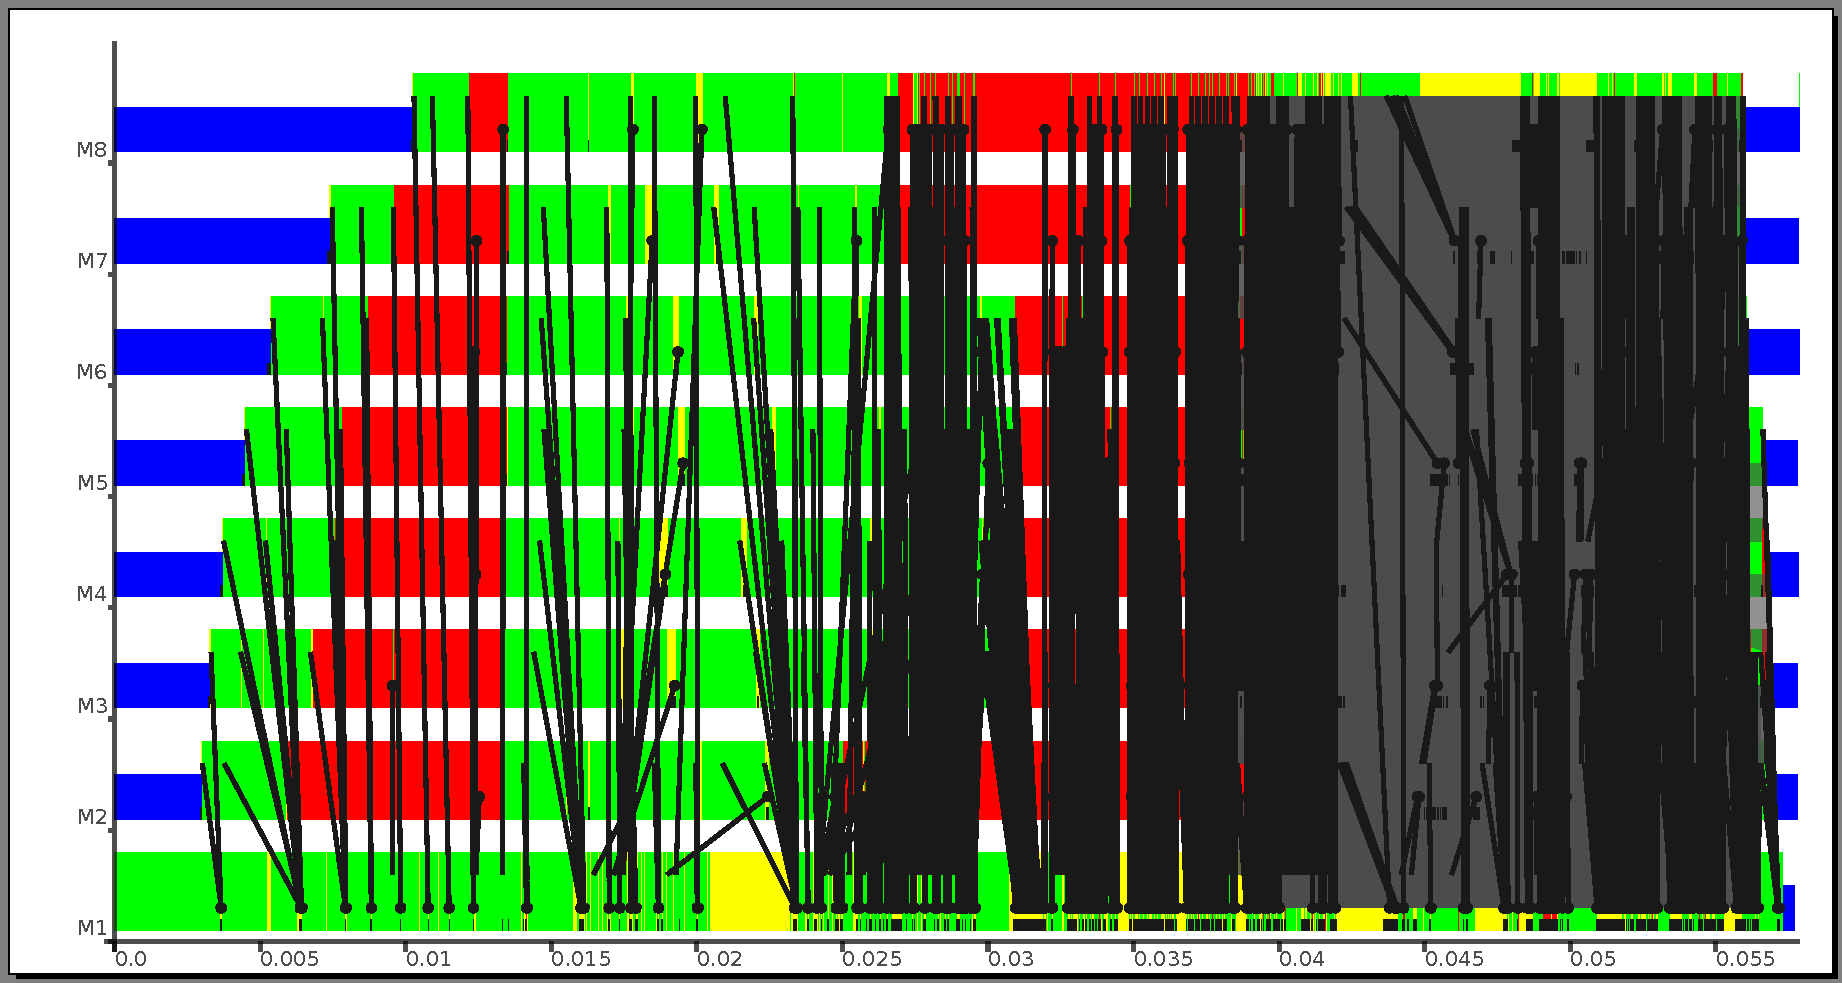
\includegraphics[width=0.9\textwidth]{images/torus_matrix_parrows_scale}
	\caption[Matrix Multiplication with a torus (Parrows)]{Matrix Multiplication with a torus (Parrows)}
	\label{fig:torus_parrows_trace}
\end{figure}

\begin{figure}[ht]
	\centering
	\includegraphics[width=0.9\textwidth]{images/torus_matrix_eden_scale}
	\caption[Matrix Multiplication with a torus (Eden)]{Matrix Multiplication with a torus (Eden)}
	\label{fig:torus_eden_trace}
\end{figure}

\FloatBarrier

%%% Local Variables:
%%% mode: latex
%%% TeX-master: "main"
%%% End:
	%\pagebreak
	\section{Benchmarks}
\label{sec:benchmarks}


%\begin{figure}[ht]
%	\centering
	\framebox{
		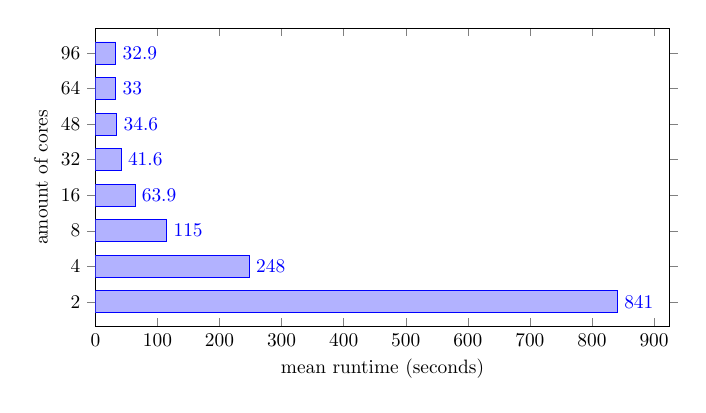
\begin{tikzpicture}[thick, scale=0.7]
		\begin{axis}[
			xbar, xmin=0,
			bar width=0.4cm,
			width=12cm, height=7cm, enlarge y limits=0.1,
			ylabel={amount of cores},
			xlabel={mean runtime (seconds)},
			symbolic y coords={2, 4, 8, 16, 32, 48, 64, 96},
			ytick=data,
			nodes near coords, nodes near coords align={horizontal},
			]
			\addplot coordinates {(841,2) (248,4) (115,8) (63.9,16) (41.6,32) (34.6,48) (33.0,64) (32.9,96)};
		\end{axis}
		\end{tikzpicture}
	}
%	\caption[Parallel Matrix Multiplication using Eden (two 1024x1024 matrices)]
%\end{figure}

\framebox{
	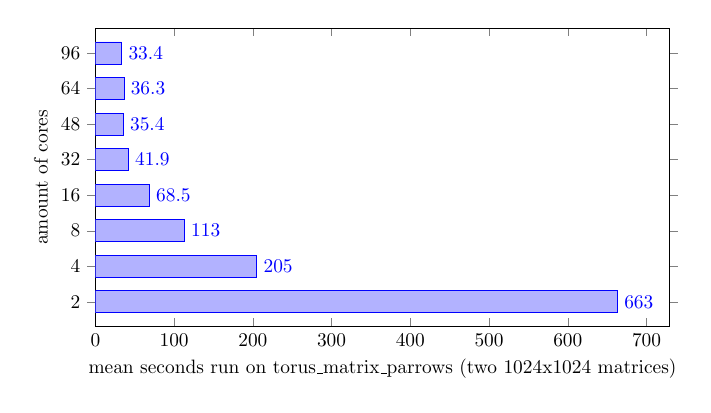
\begin{tikzpicture}[thick, scale=0.7]
	\begin{axis}[
	xbar, xmin=0,
	bar width=0.4cm,
	width=12cm, height=7cm, enlarge y limits=0.1,
	ylabel={amount of cores},
	xlabel={mean seconds run on torus\_matrix\_parrows (two 1024x1024 matrices)},
	symbolic y coords={2, 4, 8, 16, 32, 48, 64, 96},
	ytick=data,
	nodes near coords, nodes near coords align={horizontal},
	]
	\addplot coordinates {(663,2) (205,4) (113,8) (68.5,16) (41.9,32) (35.4,48) (36.3,64) (33.4,96)};
	\end{axis}
	\end{tikzpicture}
}


%%% Local Variables:
%%% mode: latex
%%% TeX-master: "main"
%%% End:
	%%\pagebreak
	\section{Conclusion}
\label{sec:conclusion}
Arrows are a generic concept that allows for powerful composition combinators. To our knowledge we are the first ones to represent parallel computation with arrows.\olcomment{that strange arrows-based robot interaction paper from 1993 or so! clearly discuss in related work}

Arrows turn out to be a useful tool for composing in parallel programs. We do not have to introduce new monadic types that wrap the computation. Instead use arrows just like regular sequential pure functions. 
%
This work features multiple parallel backends: the already available parallel Haskell flavours. Parallel Arrows feature an implementation of the \inlinecode{ArrowParallel} interface for Multicore Haskell, \inlinecode{Par} monad, and Eden. With our approach parallel programs can be ported across these flavours with no effort.
%
%
Performancewise, Parallel Arrows are on par with existing parallel Haskells, as they do not introduce any notable overhead.\olcomment{PROOFS. Many proofs in benchmarks!}

\mbcomment{ArrowApply (or equivalent) are needed because we basically want to be able to produce intermediary results, this is by definition of the parallel evaluation combinators}

\olcomment{Remove websites from citations, put them into footnotes!}

\olcomment{Parrows + accelerate = love? Metion port to Frege. Mention the Par monad troubles.}
	%\pagebreak
        \bibliographystyle{jfp}
	\bibliography{references,main}
        \appendix
	\section{Utility Functions}\label{utilfns}
To be able to go into detail on parallel arrows, we introduce some utility combinators first, that will help us later: \inlinecode{map}, \inlinecode{foldl} and \inlinecode{zipWith} on arrows.

The \inlinecode{mapArr} combinator (Fig.~\ref{fig:mapArr}) lifts any arrow \inlinecode{arr a b} to an arrow \inlinecode{arr [a] [b]} \cite{programming_with_arrows}:
\begin{figure}[h]
\begin{lstlisting}[frame=htrbl]
mapArr :: ArrowChoice arr => arr a b -> arr [a] [b]
mapArr f =
	arr listcase >>>
	arr (const []) pipepipepipe (f *** mapArr f >>> arr (uncurry (:)))
	where listcase [] = Left ()
	      listcase (x:xs) = Right (x,xs)
\end{lstlisting}
\caption{\inlinecode{map} over arrows}
\label{fig:mapArr}
\end{figure}
Similarly, we can also define \inlinecode{foldlArr} (Fig.~\ref{fig:foldlArr}) that lifts any arrow \inlinecode{arr (b, a) b} with a neutral element \inlinecode{b} to \inlinecode{arr [a] b}:
\begin{figure}[h]
\begin{lstlisting}[frame=htrbl]
foldlArr :: (ArrowChoice arr, ArrowApply arr) => arr (b, a) b -> b -> arr [a] b
foldlArr f b =
	arr listcase >>>
	arr (const b) pipepipepipe
		(first (arr (\a -> (b, a)) >>> f >>> arr (foldlArr f)) >>> app)
	where listcase [] = Left []
	      listcase (x:xs) = Right (x,xs)
\end{lstlisting}
\caption{\inlinecode{foldl} over arrows}
\label{fig:foldlArr}
\end{figure}
\fixme{pipepipepipe does not work with lhs2TeX}
Finally, with the help of \inlinecode{mapArr} (Fig.~\ref{fig:mapArr}), we can define \lstinline{zipWithArr} (Fig.~\ref{fig:zipWithArr}) that lifts any arrow \inlinecode{arr (a, b) c} to an arrow \inlinecode{arr ([a], [b]) [c]}.
\begin{figure}[h]
\begin{lstlisting}[frame=htrbl]
zipWithArr :: ArrowChoice arr => arr (a, b) c -> arr ([a], [b]) [c]
zipWithArr f = (arr $ \(as, bs) -> zipWith (,) as bs) >>> mapArr f
\end{lstlisting}
\caption{\inlinecode{zipWith} over arrows}
\label{fig:zipWithArr}
\end{figure}
 %$ %% formatting
These combinators make use of the \inlinecode{ArrowChoice} type class which provides the \inlinecode{(\textpipe\textpipe\textpipe)} combinator. It takes two arrows \inlinecode{arr a c} and \inlinecode{arr b c} and combines them into a new arrow \inlinecode{arr (Either a b) c} which pipes all \inlinecode{Left a}'s to the first arrow and all \inlinecode{Right b}'s to the second arrow.
\begin{figure}[h]
\begin{lstlisting}[frame=htrbl]
(\text{\tt pipepipepipe}) :: ArrowChoice arr a c -> arr b c -> arr (Either a b) c
\end{lstlisting}
\caption{Type signature of \inlinecode{(\textpipe\textpipe\textpipe)}}
\label{fig:codeSigPipePipePipe}
\end{figure}
\fixme{pipepipepipe does not work with lhs2TeX}

With the zipWithArr combinator we can also write a combinator \inlinecode{listApp} (Fig.~\ref{fig:listApp}), that lifts a list of arrows \inlinecode{[arr a b]} to an arrow \inlinecode{arr [a] [b]}.
\begin{figure}[h]
\begin{lstlisting}[frame=htrbl]
listApp :: (ArrowChoice arr, ArrowApply arr) => [arr a b] -> arr [a] [b]
listApp fs = (arr $ \as -> (fs, as)) >>> zipWithArr app
\end{lstlisting}
\caption{Definition of \inlinecode{listApp}}
\label{fig:listApp}
\end{figure}
% $ %% formatting
. Note that  this additionally makes use of the \inlinecode{ArrowApply} typeclass that allows us to evaluate arrows with \inlinecode{app :: arr (arr a b, a) c}.

% $ %% formatting


%%% Local Variables:
%%% mode: latex
%%% TeX-master: "main"
%%% End:
\end{document}
